% IWAI 2026 submission: Springer LNCS format, max 12 pages (incl. figures,
% excl. references) + appendix of up to 12 pages, double-blind.
\documentclass[runningheads]{llncs}

% ---------- encoding & fonts ----------
\usepackage[T1]{fontenc}
\usepackage[utf8]{inputenc}
\usepackage[expansion=false]{microtype}

% ---------- math ----------
\usepackage{amsmath}
\usepackage{amssymb}
\usepackage{mathtools}

% ---------- figures ----------
\usepackage{graphicx}
\graphicspath{{figures/}}
\usepackage{tikz}
\usetikzlibrary{calc,positioning,arrows.meta}
\usepackage{subcaption}
\usepackage{xcolor}

% ---------- layout ----------
% (LNCS fixes the text block; geometry must not be loaded)
\usepackage[numbers,sort&compress]{natbib}
\usepackage{hyperref}
\hypersetup{hidelinks}

% ---------- shorthands ----------
\newcommand{\KL}[2]{D_{\mathrm{KL}}\!\left[#1\,\middle\|\,#2\right]}
\newcommand{\E}[1]{\mathbb{E}\!\left[#1\right]}
\newcommand{\Eq}[2]{\mathbb{E}_{#1}\!\left[#2\right]}
\newcommand{\Var}[2]{\mathrm{Var}_{#1}\!\left[#2\right]}
\newcommand{\desc}{\mathrm{desc}}
\newcommand{\rw}{\rightsquigarrow}
\newcommand{\Top}{\mathsf{T}}          % propagation operator
\newcommand{\bone}{\mathbf{1}}         % unit source vector

% ---------- palette ----------
\definecolor{costc}{RGB}{40,80,170}
\definecolor{newc}{RGB}{200,120,30}      % proposed / new node (amber)

% ---------- network figure macros ----------
\tikzset{
  bel/.style={circle,draw=black!70,line width=0.4pt,minimum size=7mm,inner sep=0pt,font=\small},
  obs/.style={rectangle,draw=black!45,fill=white,minimum size=2.6mm,inner sep=0pt},
  core/.style={line width=0.9pt,black!75},
  belt/.style={line width=0.5pt,black!55},
  sens/.style={dashed,line width=0.4pt,black!40},
  anno/.style={font=\scriptsize\itshape,text=black!75,align=center},
  annoarrow/.style={-{Stealth[length=1.4mm]},line width=0.3pt,black!55},
  % directed dependency edges; the *c variants shorten to clear 7mm nodes drawn at coordinates
  dcore/.style={-{Stealth[length=1.5mm]},line width=0.9pt,black!75},
  dbelt/.style={-{Stealth[length=1.3mm]},line width=0.5pt,black!55},
  dcorec/.style={dcore,shorten <=0.37cm,shorten >=0.37cm},
  dbeltc/.style={dbelt,shorten <=0.37cm,shorten >=0.37cm},
}
\newcommand{\Positions}{%
  \coordinate (A) at (0,1.1);   \coordinate (B) at (-1.1,0);
  \coordinate (C) at (1.1,0);   \coordinate (D) at (0,-1.1);
  \coordinate (b1) at (-1.45,1.95); \coordinate (b2) at (1.45,1.95);
  \coordinate (b3) at (-2.25,0);    \coordinate (b4) at (2.25,0);
  \coordinate (b5) at (-1.45,-1.95);\coordinate (b6) at (1.45,-1.95);
  \coordinate (o1) at (-1.95,2.6);  \coordinate (o2) at (1.95,2.6);
  \coordinate (o3) at (-3.1,0);     \coordinate (o4) at (3.1,0);
  \coordinate (o5) at (-1.95,-2.6); \coordinate (o6) at (1.95,-2.6);
}
\newcommand{\Edges}{%
  \draw[dcorec] (A)--(B); \draw[dcorec] (A)--(C); \draw[dcorec] (A)--(D);
  \draw[dcorec] (B)--(C); \draw[dcorec] (B)--(D); \draw[dcorec] (C)--(D);
  \draw[dbeltc] (A)--(b1); \draw[dbeltc] (A)--(b2);
  \draw[dbeltc] (B)--(b3); \draw[dbeltc] (C)--(b4);
  \draw[dbeltc] (D)--(b5); \draw[dbeltc] (D)--(b6);
  \draw[sens] (b1)--(o1); \draw[sens] (b2)--(o2); \draw[sens] (b3)--(o3);
  \draw[sens] (b4)--(o4); \draw[sens] (b5)--(o5); \draw[sens] (b6)--(o6);
  \node[obs] at (o1){}; \node[obs] at (o2){}; \node[obs] at (o3){};
  \node[obs] at (o4){}; \node[obs] at (o5){}; \node[obs] at (o6){};
}
% tiny 3-node paradigm DAG inside an agent circle at (#1,#2)
\newcommand{\miniNet}[2]{%
  \draw[black!70,line width=0.5pt,fill=white] (#1,#2) circle (0.46);
  \fill[costc!75] ($(#1,#2)+(0,0.22)$) circle (0.055);
  \fill[costc!75] ($(#1,#2)+(-0.22,-0.13)$) circle (0.055);
  \fill[costc!75] ($(#1,#2)+(0.22,-0.13)$) circle (0.055);
  \draw[costc!80,line width=0.4pt,-{Stealth[length=1mm]}] ($(#1,#2)+(0,0.22)$) -- ($(#1,#2)+(-0.22,-0.13)$);
  \draw[costc!80,line width=0.4pt,-{Stealth[length=1mm]}] ($(#1,#2)+(0,0.22)$) -- ($(#1,#2)+(0.22,-0.13)$);
  \draw[costc!80,line width=0.4pt,-{Stealth[length=1mm]}] ($(#1,#2)+(-0.22,-0.13)$) -- ($(#1,#2)+(0.22,-0.13)$);
}

% ======================================================================
\title{Changing a Networked Mind: Paradigm Dynamics as Structure Learning over a Hidden World}
\titlerunning{Changing a Networked Mind}
% ----- ANONYMIZED for double-blind review. Restore for camera-ready: -----
% \author{Jonas Hallgren\inst{1} \and David Hyland\inst{2} \and Mahault Albarracin\inst{3}}
% \authorrunning{J. Hallgren et al.}
% \institute{Affiliation 1 \email{...} \and Affiliation 2 \and Affiliation 3}
\author{Anonymous Submission}
\authorrunning{Anonymous Submission}
\institute{Anonymous Institution(s)}
% ======================================================================

\begin{document}
\maketitle

\begin{abstract}
How does a scientific community change its mind---not about a fact, but about the \emph{frame} its
facts live in? We model a paradigm as a directed network of commitments and a community as bounded
active-inference agents who must \emph{learn} that network's structure while valuing some
conclusions over others and pooling beliefs with peers. Driving this community through the full
Kuhnian cycle, one signature organizes everything we find: \emph{conflict
resolves into confident compromise}. Valuing a conclusion shifts where beliefs settle but never
delays their yielding; under any contact, communities converge; the lone discoverer of a new
dimension is averaged away. These are theorems of the regime, not accidents of
parameters---Gaussian beliefs under precision-weighted pooling can neither reject a conflicting
source nor sustain a school. Two results measure the regime and its boundary. First, the
\emph{homogeneity effect}: in a world that genuinely supports two readings, separated
communities learn two crisply different paradigm networks, and contact under default pooling
collapses them into one blurry compromise net no member holds---averaging can never create an
edge absent from every individual. Second, infer the one quantity the defaults hold
constant---each source's \emph{reliability}, read off surprise---and distinctness returns: an
agent's confidence can fall under contradiction, and two wirings survive full contact, provided
trust reads \emph{wiring} rather than opinions. But the gate adds no new fixed point, so what it
buys, it buys as time: schools become metastable, never stable. What buys a wall is
representational: agents that carry candidate wirings and a posterior over them---fusing
within frames, communicating hypotheses rather than averaging them---hold two internally
certain camps at a genuine fixed point. Gates buy time; represented rivals buy walls.
Averaging refines a frame; it cannot grow a new one.

\keywords{Active inference \and Structure learning \and Belief sharing \and Paradigm change \and Social epistemology}
\end{abstract}

% ======================================================================
\section{Introduction: changing a frame, not a credence}
\label{sec:background}
% ======================================================================

If we want science to keep going well, goodwill is not enough: we need to know how science
\emph{works}---what kind of agent can do science at all, how a community comes to represent a
genuinely new dimension of the world, and how it loses information it once held. The question has
lately acquired a second audience, because communities of reasoning agents are no longer only
studied but \emph{built}---machine-mediated research pipelines, automated literature synthesis,
multi-agent learning systems---and every such community commits, in its aggregation step, to an
answer it rarely examines: what happens to the member who disagrees. Machine learning has begun
to name the property at stake \emph{open-endedness}, the capacity of a system to keep producing
artifacts that are novel and learnable, identified both as a grand challenge
\citep{stanley2017oe} and as an essential ingredient of any general intelligence
\citep{hughes2024}; social epistemology has long catalogued its failure modes, echo chambers
\citep{nguyen2018} and premature consensus \citep{zollman2010}. What neither supplies is a
foundation: a model of a \emph{community} of structure-learning agents explicit enough that one
can prove which aggregation dynamics preserve open-endedness and which foreclose it. This paper
builds that foundation, and its central result is a negative one with constructive content: the
most natural baseline---Gaussian beliefs under precision-weighted pooling---provably lacks the
capacity, and even the cheapest repair the failure itself names---inferring each source's
reliability from surprise---restores distinctness only as a timescale, never as a wall; a wall
appears only when the rival itself is represented, which we demonstrate at the smallest scale
that exhibits it. Averaging refines a frame; it cannot grow a new one.

To change one's mind about a fact is to update a belief; to change a paradigm is to change the
\emph{frame} in which beliefs are posed. A frame is not a credence but a \emph{structure}: a
network of conditional dependencies through which information propagates. A community that revised
only its credences, leaving the network fixed, could never change frame at all. This is the
phenomenon Kuhn named but could not run forward \citep{kuhn1962}: nothing in \emph{The Structure of
Scientific Revolutions} says, mechanistically, why a community holds a structure of commitments
long past the first disconfirming evidence, nor what finally makes the holding give way.

When the chemical community gave up phlogiston it did not revise a single credence. It rewrote a
network of commitments in which combustion, calcination, respiration, and the theory of acids were
all load-bearing on a hub that had to go: late-phlogistic theorists proposed cascading revisions that
proved mutually incompatible \citep{blumenthal2017,holmes2000}, defending less a hypothesis about
combustion than a constellation of entangled commitments \citep{boantza2011}. Phlogiston was
load-bearing for too much.

Network epistemology, the dominant formalism for such communities, cannot represent this case:
its agents hold a scalar credence in a fixed proposition and update it on a trust graph
\citep{zollman2010,oconnor2019,zollman2013,jonard2025,michelini2023}, but the phlogiston puzzle
is not a failure to converge on a number---the commitments were \emph{entangled}, and the
dispute was over which entanglements to keep. Thagard's ECHO \citep{thagard1989,thagard1990}
captures the structural intuition as undirected coherence but lacks the directed dependencies
and the expand/reduce asymmetry derived below; active-inference accounts supply precision-based
lock-in \citep{albarracin2022}, warnings that naive aggregation degrades collective precision
\citep{friston2023federated,waade2025}, and a single-agent variational cost of mind-change
\citep{hyland2025}. What none of these does is make \emph{belief structure itself} the object
of inference: a scalar credence can never say how revising one commitment forces a re-reading
of the rest---agents can herd on a number or split over it, but they cannot come to hold
different \emph{kinds} of world.

This paper lets a piece of \emph{structure} travel, so that one agent can come to represent a
commitment its peers do not. Its agents carry a directed network of commitments and learn that
network by Bayesian model expansion and reduction; they are \emph{bounded}, sampling a complex
world through narrow channels, valuing some conclusions over others, and judging what they
receive against their own model. Section~\ref{sec:bmebmr} assembles this community from the
field's own default choices; Section~\ref{sec:results} drives it through the full Kuhnian
cycle---normal science, anomaly, crisis, reduction, discovery---and opens with why one signature
had to organize everything found there: two classical theorems under which the regime can neither
reject a conflicting source nor sustain a school, so that \emph{conflict resolves into confident
compromise}. Two results then measure the regime and its boundary: the \emph{homogeneity
effect}---separated communities learn genuinely different paradigm networks, and any contact
under default pooling collapses them into a compromise no one holds---and its repair, in two
stages: track each source's reliability as a latent and distinctness returns as a timescale;
represent the rival itself---candidate wirings, a posterior over them, hypotheses communicated
rather than averaged---and it returns as a wall. The discussion draws the map: what filling
the representational slot bought, and what remains.
The story, compactly, is about averaging---what belief revision is when value enters as a tilt
rather than a stiffness, what propagation-by-averaging does to a population of structure
learners, and what it takes for multi-agent structure learning to be \emph{open-ended} rather
than self-sealing.

% ======================================================================
\section{What a model of science must contain}
\label{sec:hidden}
% ======================================================================

Three things, at least. \emph{Structure as the object of inference}: a scientist confronting a
new domain is not given the right variables, let alone the dependencies among them; frames
differ in kind, not in degree, so credences over a fixed menu cannot carry them
\citep{ullman2020,kemp2008form,ullman2012}. Once structure is the object, exploration stops
being a hand-tuned bonus \citep{zollman2010,oconnor2019} and becomes the epistemic value of
\emph{expanding} the model to entertain a commitment not yet in it
\citep{friston2015,friston2017curiosity}, with Bayesian model reduction as its complement,
pruning what the data abandon in closed form \citep{friston2018bmr,neacsu2022}. Existing
applications of that machinery run on single agents \citep{neacsu2022,priorelli2023} or define
``group'' as between-subject neuroimaging \citep{friston2016peb}; a \emph{community} jointly
expanding and reducing a paradigm is the open move this paper makes.

\emph{Value}, because scientists care about their conclusions: a result on which a career rests
is held more tightly than its evidence warrants \citep{kitcher1990,strevens2003}, and attitudes
demonstrably live on networks of exactly this kind \citep{dalege2016}. And \emph{communication},
because science is social: beliefs travel a trust graph and must somehow be combined when they
meet. Each requirement has a default formalization, so natural it is hardly ever examined.
Beliefs over a network become a precision-weighted Gaussian model; value becomes a utility that
tilts the prior \citep{hyland2025}; combination becomes precision-weighted averaging, the
information form of classical opinion pooling \citep{degroot1974,genest1986}.
Section~\ref{sec:bmebmr} builds the community out of exactly these defaults, on purpose. The
question the rest of the paper asks is whether such a community can ever do more than
\emph{refine}: whether agents built this way can grow a frame, and not merely polish the one
they hold.

% ======================================================================
\section{The model}
\label{sec:bmebmr}
% ======================================================================

We draw the system whole first---a population of agents on a trust graph---then build the single
agent up from first principles, and finish by stating the dynamics as an explicit per-round loop
(\S\ref{sec:model}).

\subsection{The population, and the paradigm network each agent carries}
\label{sec:carryover}

The third requirement of \S\ref{sec:hidden}---communication---fixes the shape of the whole, so we
draw the whole first. A population of $N$ agents inhabits a shared hidden world. Agents are
coupled on a trust graph: communities are blocks of a stochastic block model, with dense
intra-community edges and an inter-community coupling weight (\emph{inter}) that we sweep from
total isolation to dense contact. Each agent privately carries its own \emph{paradigm network}, a directed graph
$G=(V,E,\Pi)$: nodes carry theoretical commitments $x_v$, edges carry inferential dependencies,
and each edge bears a coupling precision $\pi_{uv}$ measuring how tightly $v$ is bound to
$u$---from which the agent's conservatism and conviction will be derived (Eqs.~\ref{eq:kappa}
and~\ref{eq:U} below). Figure~\ref{fig:population} draws the picture.

\begin{figure}[h!]
\centering
\resizebox{0.78\linewidth}{!}{%
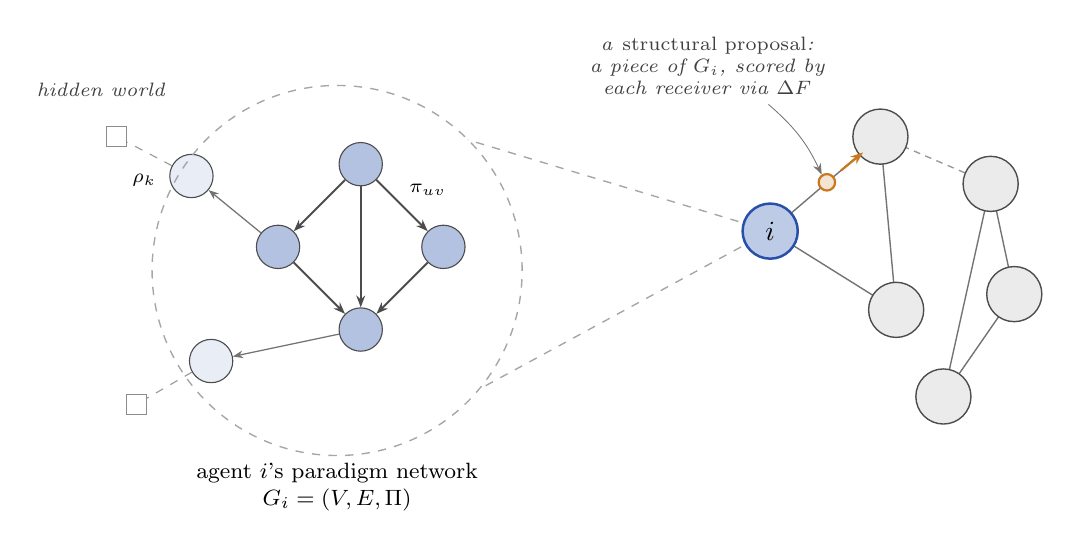
\begin{tikzpicture}[
  n/.style={circle,draw=black!70,line width=0.4pt,fill=costc!35,minimum size=5.5mm,inner sep=0pt},
  nb/.style={circle,draw=black!70,line width=0.4pt,fill=costc!10,minimum size=5.5mm,inner sep=0pt},
  ag/.style={circle,draw=black!70,line width=0.5pt,fill=black!8,minimum size=7mm,inner sep=0pt},
  dep/.style={-{Stealth[length=1.5mm]},line width=0.7pt,black!70},
  depb/.style={-{Stealth[length=1.3mm]},line width=0.45pt,black!55}]
  % ---- left: agent i's paradigm network, magnified ----
  \node[n] (A) at (0,1.05) {};
  \node[n] (B) at (-1.05,0) {};
  \node[n] (C) at (1.05,0) {};
  \node[n] (D) at (0,-1.05) {};
  \node[nb] (b1) at (-2.15,0.9) {};
  \node[nb] (b2) at (-1.9,-1.45) {};
  \draw[dep] (A)--(B); \draw[dep] (A)--(C); \draw[dep] (A)--(D);
  \draw[dep] (B)--(D); \draw[dep] (C)--(D);
  \draw[depb] (B)--(b1); \draw[depb] (D)--(b2);
  \node[obs] (o1) at (-3.1,1.4) {};
  \node[obs] (o2) at (-2.85,-2.0) {};
  \draw[sens] (b1)--(o1); \draw[sens] (b2)--(o2);
  \node[font=\scriptsize] at (0.85,0.72) {$\pi_{uv}$};
  \node[font=\scriptsize] at (-2.75,0.85) {$\rho_k$};
  \node[anno] at (-3.3,2.0) {hidden world};
  % the agent's boundary, pierced by its sensory channels
  \draw[black!35,dashed,line width=0.5pt] (-0.3,-0.3) circle (2.35);
  \node[font=\footnotesize,align=center] at (-0.3,-3.05)
    {agent $i$'s paradigm network\\$G_i=(V,E,\Pi)$};
  % ---- magnifier lines to one agent of the trust graph ----
  \draw[black!35,dashed,line width=0.5pt] (5.2,0.2) -- (1.36,1.36);
  \draw[black!35,dashed,line width=0.5pt] (5.2,0.2) -- (1.5,-1.81);
  % ---- right: the trust graph, two communities ----
  \draw[belt] (5.2,0.2)--(6.6,1.4); \draw[belt] (5.2,0.2)--(6.8,-0.8);
  \draw[belt] (6.6,1.4)--(6.8,-0.8);
  \draw[belt] (8.0,0.8)--(8.3,-0.6); \draw[belt] (8.3,-0.6)--(7.4,-1.9);
  \draw[belt] (8.0,0.8)--(7.4,-1.9);
  % the single weak channel between communities
  \draw[line width=0.5pt,black!40,dash pattern=on 2.4pt off 2pt] (6.6,1.4)--(8.0,0.8);
  \node[ag,fill=costc!30,draw=costc,line width=0.9pt] (ai) at (5.2,0.2) {$i$};
  \node[ag] (a2) at (6.6,1.4) {};
  \node[ag] (a3) at (8.0,0.8) {};
  \node[ag] (a4) at (6.8,-0.8) {};
  \node[ag] (a5) at (8.3,-0.6) {};
  \node[ag] (a6) at (7.4,-1.9) {};
  % ---- the object being passed: a structural proposal ----
  \node[circle,draw=newc,line width=0.8pt,fill=newc!20,inner sep=2.1pt] (prop) at (5.92,0.82) {};
  \draw[-{Stealth[length=1.6mm]},newc,line width=0.8pt] (6.1,0.97) -- (6.38,1.2);
  \node[anno] (anProp) at (4.4,2.3) {a \emph{structural proposal}:\\a piece of $G_i$, scored by\\each receiver via $\Delta F$};
  \draw[annoarrow] (anProp) to[bend left=12] (prop);
\end{tikzpicture}}
\caption{The population model. Right: a trust graph, fixed at the start (stochastic block
model)---dense channels within a community, one weak weight \emph{inter} between. Left,
magnified: each agent's private paradigm network $G_i=(V,E,\Pi)$, its belt reading the hidden
world through channels of precision $\rho_k$. Along trust channels travel fused posteriors and
\emph{structural proposals}: pieces of paradigm each receiver scores against its own net by
$\Delta F$ (Eq.~\ref{eq:bmr}).}
\label{fig:population}
\end{figure}

Two kinds of things propagate on this underlying network. Beliefs and accumulated precisions are
fused across trust edges in information form---a precision-weighted pooling of posteriors in which
an agent's own evidence and its neighbours' carry weight in proportion to trust, the
information-form counterpart of trust-weighted averaging in opinion dynamics
\citep{degroot1974,acemoglu2011}. And---this part is not standard---\emph{structure} spreads the
same way: an agent whose neighbour has awakened a new node receives the proposal and scores it
against its own model (\S\ref{sec:structurelearning}). What travels on the trust graph is not only
a number but a piece of structure, evaluated against wiring the sender does not see.

What does one of those private networks hold? Begin concretely. The
phlogiston paradigm, at its smallest, is three commitments wired together:
combustion releases phlogiston; calcination is combustion, slowed; respiration is combustion,
tamed. Each commitment conditions the next, evidence for any one bears on all, and the question
``what if the calx \emph{gains} weight?'' has no local answer---it tugs the whole web. A
paradigm, in this paper, is that web made explicit.

The network is just a generative model whose hidden states are the commitments themselves:
internal coherence is the precision-weighted graphical model $p(x\mid
G)\propto\prod_{(u\to v)\in E}\psi_{uv}(x_u,x_v)^{\pi_{uv}}$---a linear-Gaussian structural
equation model in the lineage of Wright's path analysis \citep{wright1934}, edges as path
coefficients and precisions as their weights. We work throughout in that regime, which puts
every quantity below in closed form (Appendix~\ref{app:operator}); agents are
\emph{honest}---no one misreports, so lock-in is never a dishonesty artifact---and
\emph{bounded}, minimizing variational free energy step by step \citep{dacosta2020}.

Revising a commitment is not a local act: changing $x_v$ forces everything downstream to
re-equilibrate, along every chain of dependence. If $A$ is the matrix of edge precisions,
summing chains of every length gives $\sum_k A^k=(I-A)^{-1}$---a finite sum on a DAG, an object
two literatures already own: the \emph{total-effects matrix} of path analysis
\citep{wright1934,bollen1987}, the Katz--Bonacich index of network science
\citep{katz1953,bonacich1987,malioutov2006}. We adopt it as the \emph{propagation operator}
$\Top=(I-A)^{-1}$: the entry $\Top_{iw}=\pi_{i\rw w}$ is the total precision-weighted coupling
propagated from $i$ to $w$ along all directed paths (Appendix~\ref{app:operator}).

Conservatism is then recognized rather than posited. Place a unit of weight on every node and ask,
for each commitment $i$, how much total weight a revision of $i$ would disturb. That is the operator
applied to the unit source,
\begin{equation}
\kappa \;=\; \Top\,\bone,
\qquad
\kappa_i \;=\;1+\!\!\sum_{w\in\desc(i)}\!\!\pi_{i\rw w},
\label{eq:kappa}
\end{equation}
the precision-weighted mass of a node's descendants. In network-science terms this is a
centrality (the broadcast Katz index), usually read as influence or status; we read the same
number as \emph{revision cost}---a commitment is exactly as expensive to revise as the mass that
must re-equilibrate when it moves. Conservatism is a centrality the graph already determines,
not a disposition assigned by hand.

What we add to this inherited machine comes in two layers. The first is contact with the world. The
dense, high-precision interior of the network is the \emph{core}; the sparse periphery in contact
with observation is the \emph{belt}, each belt node reading the world through a sensory channel of
precision $\rho_k$. The core carries no direct sensory channel: an interior commitment is revised
only by error propagated inward from the belt, through the same operator---costly by
Eq.~\eqref{eq:kappa} and insulated by position, which is what makes it slow.

The second layer is value, and the operator is run twice. Scientists value some conclusions over
others (\S\ref{sec:hidden}); following the variational-cost account of belief
revision \citep{hyland2025}, we attach to each node an intrinsic utility $u_i$ and let it propagate
through the \emph{same} operator: a commitment one wants true lends value to its dependents, so the
conviction field is
\begin{equation}
U \;=\; \Top\,u,
\qquad
U_i \;=\; u_i+\!\!\sum_{w\in\desc(i)}\!\!\pi_{i\rw w}\,u_w .
\label{eq:U}
\end{equation}
In the operator's path-analytic reading, $U$ is the total effect of wanting things true. Where the
inherited models propagate a single source, a paradigm carries two: $\Top\bone$ and $\Top u$ are
linearly independent unless $u\propto\bone$, so the two fields need not align---a commitment can
be central yet value-neutral, cheap yet strongly held (Fig.~\ref{fig:twofields},
Appendix~\ref{app:operator}).

\subsection{Motivated revision and the lock-in parameter}
\label{sec:revision}

The bounded agent revises its belief $q(x)$ over the whole network by the motivated trade of
\citet{hyland2025}: the variational cost of changing its mind---divergence from the prior its own
Bayes net encodes---against accuracy to the evidence and the value of where the commitments land,
\begin{equation}
\begin{aligned}
\mathcal{F}[q]\;&=\;
\underbrace{\KL{q(x)}{p(x\mid G)}}_{\text{mind-change cost}}
\;-\;\underbrace{\Eq{q}{\log p(o\mid x,G)}}_{\text{accuracy}}
\;-\;\lambda\,\underbrace{\Eq{q}{U^{\!\top}\!x}}_{\text{value}}\\[2pt]
&\Longrightarrow\qquad
q_\lambda(x)\;\propto\;p(x\mid o,G)\,e^{\lambda\,U^{\!\top}\!x},
\end{aligned}
\label{eq:tilted}
\end{equation}
with $\lambda$ a single temperature governing how far value may bend the evidence. The KL is
anchored to the \emph{network prior}: mind-change is priced from where the mind currently
stands, in the metric of the paradigm's own precision (Appendix~\ref{app:operator},
Eq.~\ref{eq:mindcost}), and the minimizer is classical---the exponential tilt KL-regularized
utility maximization always yields \citep{todorov2009,ortega2013}. What is ours is the source
of the tilt, a conviction field propagated through the paradigm's own operator. In the
linear-Gaussian regime the tilt is a pure mean shift, displacing the commitments by
$\lambda\Sigma U$ and leaving the covariance untouched. What opposes the displacement is
evidence, also through the mean: a disconfirming channel $k$ with sensory precision $\rho_k$
and read-out $H_k$ pulls the mean back with gain $\propto\rho_k\,H_k\Sigma U$---so as
conviction drives $\rho_k\to0$, the value-displaced commitment stands unrefuted. The fraction
of disconfirming sensory precision so silenced,
\begin{equation}
\gamma\;=\;\frac{\sum_{k\in\mathrm{dis}}\rho_k\,\mathbb{1}[\,\rho_k\ \text{gated by the core}\,]}
{\sum_{k\in\mathrm{dis}}\rho_k},
\label{eq:gamma}
\end{equation}
is the \emph{lock-in parameter}. Nothing is silenced by hand: each round channel $k$ carries
weight $w_k=\exp(-g\,|U\!\cdot\!H_k|)$---the more directly a channel bears on valued
commitments, the less the agent listens, with $g$ setting how strongly caring becomes
not-listening. Note what this mechanism \emph{is}: a displacement of where beliefs come to
rest---under forgetting a \emph{saturating} one (\S\ref{sec:temporal}) while evidence keeps
arriving. A bias, not a resistance; the results make that distinction load-bearing.

\subsection{Structure learning: reduction and expansion}
\label{sec:structurelearning}

Structure learning revises $G$ itself---the first requirement of \S\ref{sec:hidden}, that
structure be the \emph{object} of inference, now discharged by two asymmetric operations
\citep{friston2017curiosity,smith2020structure}. The asymmetry is the formal counterpart of normal
versus revolutionary science.

\emph{Reduction} is the exact half. Each edge is parameterized by a prior precision $\alpha_e$
($\alpha_e\to\infty$ pins the edge's parameter to zero; $\alpha_e\to0$ frees it), the
automatic-relevance-determination parameterization of sparse Bayesian learning
\citep{mackay1992,tipping2001}. Bayesian model reduction \citep{friston2011,friston2018bmr} scores any
pruning in closed form from the already-inverted posterior,
\begin{equation}
\frac{p(o\mid\tilde M)}{p(o\mid M)}=\Eq{p(\theta\mid o)}{\frac{\tilde p(\theta)}{p(\theta)}},
\label{eq:bmr}
\end{equation}
the Savage--Dickey ratio in general form: one inversion scores every candidate reduced structure
without re-touching the data.

\emph{Expansion} reaches what reduction cannot: a commitment no one has represented. Following
\citet{friston2017curiosity}, the agent entertains a new node by wiring it tentatively to existing
nodes with free priors ($\alpha_e\to0$) and letting reduction prune the proposal back to the couplings
the data support. Expansion is not closed-form---a new node may enlarge the
likelihood's support and requires a real inversion---and this cost asymmetry is why a field
reorganizes its periphery continually and its centre only rarely. The agent does not plan \emph{when}
to expand: candidates arrive at a Poisson rate, and an arrival is kept only if the model log Bayes
factor favours the wired-in node (Appendix~\ref{app:crisis-discovery}). It must be a rate,
because one cannot plan toward a dimension one has not yet conceived \citep{stanford2006};
Appendix~\ref{app:closing} treats the rate itself as a belief---the agent's belief that its own
model class is incomplete---with the constant rate as the agnostic baseline.

\subsection{Forgetting}
\label{sec:temporal}

Without forgetting, $\kappa=\Top\bone$ can only grow as learning adds edges: a paradigm is a
ratchet, and lock-in under it is automatic rather than earned. We import the standard remedy
unmodified: accumulated precision relaxes toward the prior, $\Pi\leftarrow\Pi_0+\omega(\Pi-\Pi_0)$
with forgetting factor $\omega\in(0,1]$ \citep{friston2017process,smith2022tutorial}---the
agent's prior on the world's structural drift; one forgets at the rate one believes the
structure is moving \citep{mathys2011}. The operator inherits the time index, and a once-central
node whose couplings go unreinforced relaxes back toward cheapness. With forgetting, the value
tilt saturates at $\lambda U/(1-\omega)$ against also-saturated per-step evidence, so conviction
holds only above a threshold---motivated persistence turned from a posited bias into a threshold
conviction must clear.

\subsection{Reliability as a latent}
\label{sec:reliability}

One default remains, so quiet it is rarely stated: every precision above is \emph{known}---the
sensory $\rho_k$, the trust weights of the fusion step---constants, blind to what the source
actually says. The results open with what that costs (two theorems; \S\ref{sec:results}), and
the conflict-resolution literature has long owned the repair \citep{ohagan2012}: stop treating
a source's precision as a constant and \emph{infer} it. Carried as a scale mixture, each
channel's noise precision becomes a latent with its own prior, and its posterior expectation,
given the standardized one-step surprise $z_k^2$ (the squared residual of observation $k$
against the agent's own prediction, in units of its predictive variance), is the classic
Student-$t$ weight
\begin{equation}
\eta_k \;=\; \frac{\nu+1}{\nu+z_k^2},
\label{eq:lambda}
\end{equation}
applied multiplicatively to the channel's evidence deposit. The rule is one sentence:
\emph{trust what does not keep surprising you}. A channel reporting on-prediction
($z^2\!\sim\!1$) keeps full weight; a gross outlier is discounted as $\nu/z^2$; the single dial
$\nu$ sets how quickly surprise becomes doubt, and $\nu\to\infty$ recovers the Gaussian
defaults exactly. The same functional gates trust \emph{between} agents,
$\eta_{ij}=(\nu_s+1)/(\nu_s+z_{ij}^2)$, with $z_{ij}^2$ the calibrated disagreement between
$i$'s and $j$'s posteriors---and because $z^2$ is just a calibrated gap, the gate can be
pointed at \emph{opinions} (the posterior means) or at \emph{wiring}, the contested coupling
entries of $\Pi$ itself (definitions in Appendix~\ref{app:reliability}). Note what the gate is
not: it adds no objective and no memory, every weight stays strictly positive, and so it
creates no new fixed point. Both gates default to off, reproducing the baseline
byte-identically.

\subsection{Represented rivals}
\label{sec:rivals}

The gate infers how much to trust a source; it cannot represent the \emph{alternative} a
source argues for. The last mechanism supplies that slot, at the smallest scale that makes it
testable. Each agent carries $K$ candidate wirings $(\Pi_k,h_k)$ and a posterior over a model
index---$q_i(x,m)$ rather than $q_i(x)$---and each step every candidate is scored by its
prequential predictive density \emph{before} the shared deposit lands, so the
structure-discriminating evidence the Fisher deposit erases accumulates in the log-weights
$L_{ik}$. Communication changes accordingly: parameter beliefs fuse only \emph{within} a frame
(candidate $k$ with neighbours' candidate $k$, never averaged across frames), and what travels
\emph{between} frames is the hypothesis itself, by damped log-linear pooling of the
log-weights, $L\leftarrow(1-\alpha_m)L+\alpha_m W L$. The damping is the point: it gives the
pooled log-odds a genuine fixed point at a constant gap set by each camp's own evidence source
(${\sim}\,s/2\alpha_m$ nats for two symmetric camps), where the gates of
\S\ref{sec:reliability} leave consensus as the only fixed point. $K=1$ reduces exactly to the
baseline's fuse-then-observe, so the comparisons of \S\ref{sec:results} run all three
architectures on byte-identical observation streams (definitions in
Appendix~\ref{app:reliability}).

% ======================================================================
\subsection{The simulation at a glance}
\label{sec:model}
% ======================================================================

The pieces are now all on the table: the population of \S\ref{sec:carryover}, each agent revising
under conviction (\S\ref{sec:revision}), learning structure (\S\ref{sec:structurelearning}), and
forgetting (\S\ref{sec:temporal}). Concretely, the experiments of \S\ref{sec:results} instantiate the phlogiston world: a hub-structured
paradigm net in which a single core commitment (phlogiston) is load-bearing for combustion,
calcination and respiration; at a fixed step $t_{\mathrm{shift}}$ the world's regime flips (the calx
is heavier---the gravimetric anomaly), and the truth thereafter contains a dimension (oxygen) that is
\emph{not in any agent's network}. One round of the simulation, for every agent:

\begin{enumerate}\itemsep1pt
\item \textbf{Observe.} The world emits observations at the belt; disconfirming channels carry
the conviction-gate weight $w_k$ (\S\ref{sec:revision}) and, with the reliability gate on, the
inferred $\eta_k$ (Eq.~\ref{eq:lambda}).
\item \textbf{Infer.} Exact linear-Gaussian update of the value-tilted posterior
(Eq.~\ref{eq:tilted}); precision accumulates.
\item \textbf{Crisis check (reduction).} Candidate prunes are scored by
$\Delta F+\lambda_i\,\Delta U$, both terms closed-form from the Savage--Dickey reduced
posterior (Eq.~\ref{eq:bmr}); both protective belt edges clearing the bar is a \emph{crisis},
and the hub is released (Appendix~\ref{app:crisis-discovery}).
\item \textbf{Discovery check (expansion).} When a Poisson proposal arrives, its direction is
read from the post-reduction residual's leading eigenvector, and the wake is kept iff the
model log Bayes factor is positive (Appendix~\ref{app:crisis-discovery};
Appendix~\ref{app:closing} makes the rate a posterior and a social process).
\item \textbf{Fuse.} Posteriors and structural edits pool across the trust graph, weighted by
the intra/inter coupling and, with the social gate on, by $\eta_{ij}$
(\S\ref{sec:reliability}); pooling all dimensions vs.\ only those jointly represented is a
protocol choice with consequences (Appendix~\ref{app:null}).
\item \textbf{Forget.} Accumulated precision decays by $\omega$ (\S\ref{sec:temporal}).
\end{enumerate}

Crisis, revolution and discovery are thus not stipulated events but threshold crossings of the
model's own evidence; Appendix~\ref{app:crisis-discovery} derives both checks from the single
tilted objective and lists explicitly what remains a modelling commitment.
Table~\ref{tab:dials} (Appendix~\ref{app:null}) lists the dials swept; everything else is held
fixed, and all code is seeded and ships its own null and positive controls.

One thing deserves emphasis before the results: every baseline ingredient above is its field's
default---Kalman-filter belief updating, the standard formalization of motivated reasoning,
classical opinion pooling in information form, textbook Bayesian model comparison. Nothing
exotic has been smuggled in; the results test what these defaults can do \emph{together}.

% ======================================================================
\section{Results}
\label{sec:results}
% ======================================================================

All results are from the population of \S\ref{sec:carryover}, run by the loop of
\S\ref{sec:model}. The main text reports two experiments, each chosen to isolate one claim at
the smallest scale that exhibits it; the full Kuhnian-cycle sweep on the phlogiston
world---crisis, reduction, and discovery as threshold crossings of the agents' own evidence,
none stipulated---is consistent with both and carried in Appendix~\ref{app:null}. One signature
organizes everything we find: \emph{conflict resolves into confident compromise}. It is not an
accident of parameters. Two classical theorems, one per level of the model, say it could not
have come out otherwise.

\emph{Pooling is a contraction.} The fusion step is precision-weighted averaging on a connected
trust graph---DeGroot dynamics in information form \citep{degroot1974}---and its weights never
depend on the \emph{content} of what is pooled. Any such step contracts the spread of beliefs
geometrically toward consensus: disagreement can only decay, never regenerate. A persistent
school of thought would require an agent to weigh a message by its fit to the agent's own
structure, and no quantity in the loop of \S\ref{sec:model} reads that fit; the hazard is
recognized within active inference itself \citep{catal2024}. \emph{Gaussian conflict resolves by
compromise.} Within an agent the same impossibility holds one level down, and it has been a
theorem for fifty years: a posterior built from light-tailed sources responds to conflict between
them by confident compromise---it can never reject a conflicting source, however extreme
\citep{dawid1973,ohagan1979}---and its precision \emph{grows} while doing so \citep{ohagan2012},
so contradiction makes a Gaussian agent more certain, never less. There is no slot in $(\Pi,h)$
for being torn: crisis as suspended confidence requires tails the regime does not have.

The two theorems make this community a \emph{null regime}---the simplest faithful model of a
believing, communicating community, in which Kuhnian phenomena provably cannot arise. But they
are qualitative: what they do not say is where the boundary sits, or how sharply it cuts. We
measure both, as two results: the homogenization the theorems demand
(\S\ref{sec:res-homogeneity}; the full characterization in Appendix~\ref{app:null}), and what
happens when the one quantity the theorems hold fixed---each source's reliability---is inferred
instead (\S\ref{sec:res-distinct}; Appendix~\ref{app:reliability}). The nets are
hand-wired to expose the geometry, not fitted to data: nothing here is evidence about chemistry,
only about how a structured, bounded, valued mind changes.

\subsection{Result 1: the homogeneity effect}
\label{sec:res-homogeneity}

The experiment is simple. The world is built so that its data admit two equally good
readings---two different ways of wiring the same commitments into a paradigm network. We split
the population into two communities and give them different values, so each community attends
to the observations that favour one of the two wirings; we then measure the \emph{structure
distance} between the networks the agents actually learn---small when two agents wire the
world the same way, large when they wire it differently. The question is whether one
population can come to hold both readings.

Kept apart, it can (Fig.~\ref{fig:res-divergence}, blue): each community settles on its own
wiring---agents within a community agree (dashed, at zero) while the distance between the two
communities grows large and stays there. Run the same world with the communities connected,
pooling beliefs every round (red), and the divergence never forms: each fusion step averages
the two half-formed wirings into one compromise network that neither community's evidence
supports, and the final distance between the camps is a tenth of what isolation produced. This
is Result 1, the \emph{homogeneity effect}: under default pooling, a connected population ends
up holding one network, whatever diversity its members were learning---not because any dial
was set against pluralism, but because the contraction theorem leaves the dynamics nowhere
else to go.

\begin{figure}[h!]
\centering
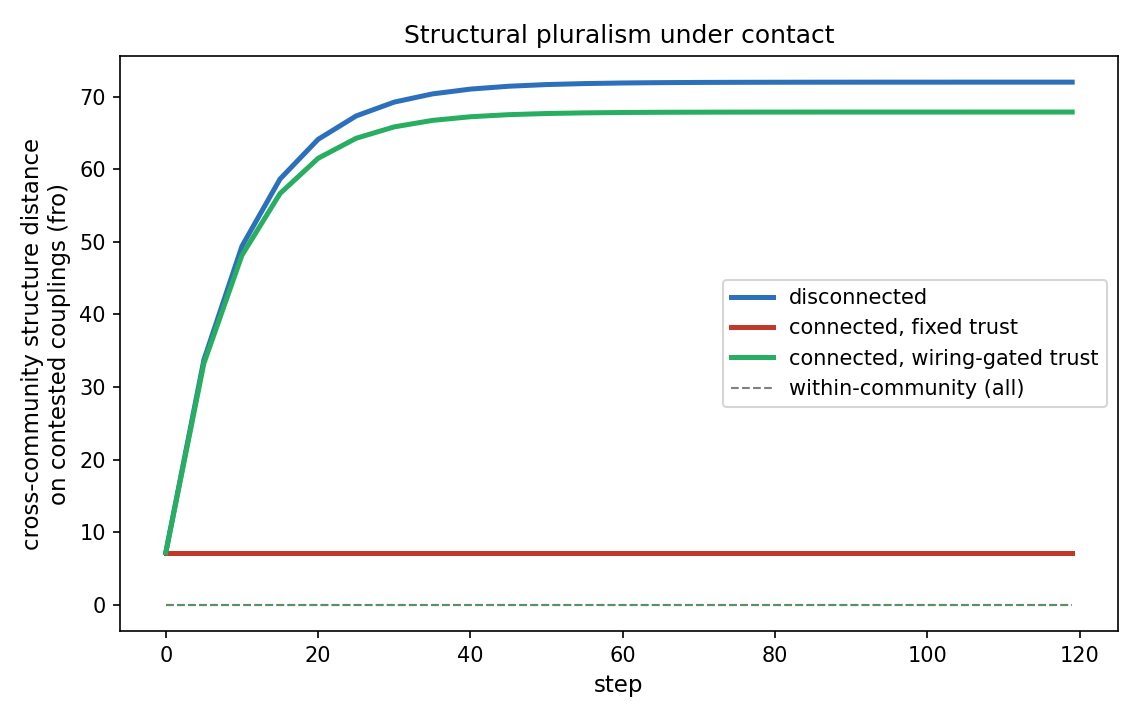
\includegraphics[width=0.8\linewidth]{fig_divergence_traces.png}
\caption{The paper's two results in one experiment (a structurally underdetermined world;
cross-community distance on the contested couplings, mean $\pm$ s.d., 5 seeds; dashed:
within-community, ${\sim}0$ throughout). Apart (blue): two crisply different wirings.
Connected, default fusion (red): the pluralism never forms---$10\%$ of the disconnected
divergence, the homogeneity effect (Result 1). Connected, wiring-reading trust (green,
\S\ref{sec:reliability}): $94\%$ survives full contact (Result 2).}
\label{fig:res-divergence}
\end{figure}

The phlogiston sweep (Appendix~\ref{app:null}) finds the same effect at every level of the
model. \emph{Conviction does not protect:} valuing a conclusion shifts where an agent's
beliefs settle, never when they yield \citep{hyland2025}; the only thing conviction can do is
make an agent stop listening to its own disconfirming channels. \emph{Isolation is the only
protection, and it is fragile:} at \emph{inter}$=0.005$---trust toward outsiders two hundred
times weaker than trust within the community---$92\%$ of a dogmatic community converts,
because what arrives from a neighbour is \emph{evidence}, and an agent can silence its own
instruments but not its neighbours'. \emph{Discovery does not survive company:} a new concept
woken by a single agent is averaged away, because peers who lack the concept treat ``has no
such variable'' as ``certainly zero.'' \emph{No added mechanism escapes:} adequacy-driven
exploration, social excitation, audited curiosity, and value accretion each re-time the
passage to consensus or synchronize the population for it; none lets two connected communities
holding the same data stay in disagreement. The effect even has a one-line algebraic face:
$|\,\mathrm{mean}_i\,\Pi_i\,|\le\max_i|\Pi_i|$ entrywise, so an average can never
\emph{create} an edge absent from every individual (measured synergy exactly zero)---whatever
a collective knows beyond its members lives in the \emph{union} of their networks, never in
their average.

\subsection{Result 2: distinctness returns---gates buy time, represented rivals buy walls}
\label{sec:res-distinct}

The same setups, the same evidence; what changes is only what the agents \emph{represent}.
First, switch on the gate of \S\ref{sec:reliability}, so that each source's reliability is
tracked as a latent instead of held constant.
Within an agent, the smallest possible setting already shows what changes
(Fig.~\ref{fig:res-variance}). One agent holds a three-commitment chain; at step $30$ one
channel turns persistently contradictory. The Gaussian baseline does what Theorem 2 says it
must: it settles confidently between the channel's report and what its own couplings imply, its
variance falling monotonically throughout---the conflict leaves \emph{no trace} in the belief
state. The gated agent instead infers the channel unreliable ($\eta$ falls to $0.16$), and
its uncertainty does something no light-tailed posterior can: it \emph{rises} while evidence
accumulates, peaking eight steps after the conflict begins, before the belief reorganizes
around the discounted channel and reliability recovers. There is now a slot in the belief
state for being torn---crisis as suspended confidence, rendered as a posterior.

\begin{figure}[h!]
\centering
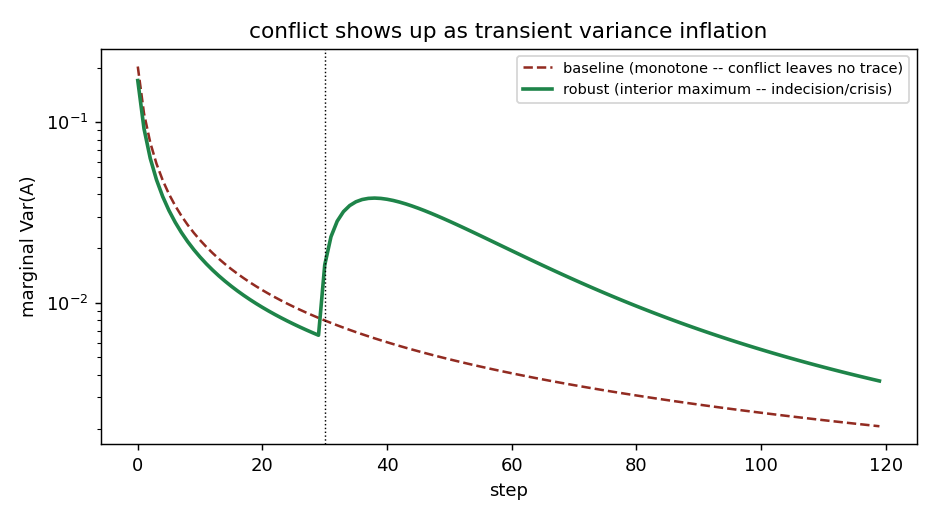
\includegraphics[width=0.52\linewidth]{fig_abc_variance.png}
\caption{Conflict as suspended confidence. A channel turns contradictory at step 30. The
Gaussian baseline (dashed) grows monotonically more certain---Theorem 2's confident
compromise; the gated agent's variance (solid) shows an interior maximum: doubt rises while
data accumulate, then resolves.}
\label{fig:res-variance}
\end{figure}

Between communities, point the same functional at the \emph{wiring}---the contested coupling
entries of $\Pi$---and the collapse of Fig.~\ref{fig:res-divergence} reverses (green curve):
two crisp wirings survive full contact, $94\%$ of the disconnected divergence retained where
fixed trust keeps $10\%$. What the gate \emph{reads} decides the outcome: pointed at
\emph{opinions} it never fires here ($10.2\%$, indistinguishable from fixed trust), because
both camps fit the same blended data and so agree in their means---a pluralism that lives in
wiring is invisible to a trust that reads opinions.

But the gate is memoryless and its weights stay strictly positive, so the contraction theorem
still owns $t\to\infty$: every school the gate sustains is metastability relative to a
horizon, not a new fixed point. Figure~\ref{fig:res-walls} makes the full hierarchy visible on
one long run. Two camps in full contact, each running only its own commitment's
experiment---theory-laden evidence, the Kuhnian condition---compared across three
architectures on byte-identical observation streams. Plain fusion collapses the disagreement
within a few steps: the theorem. The trust gate, at its best calibration, holds the gap for
hundreds of steps and then visibly decays: time, bought and spent. The rival layer of
\S\ref{sec:rivals} holds a flat gap to $t=1500$ with each camp internally certain of its own
theory ($q_{\mathrm{own}}=1.0$ on both sides): a wall---a fixed point of the damped
hypothesis-pooling dynamics, not a slow leak (the tail slope is non-eroding;
Appendix~\ref{app:reliability}).

\begin{figure}[h!]
\centering
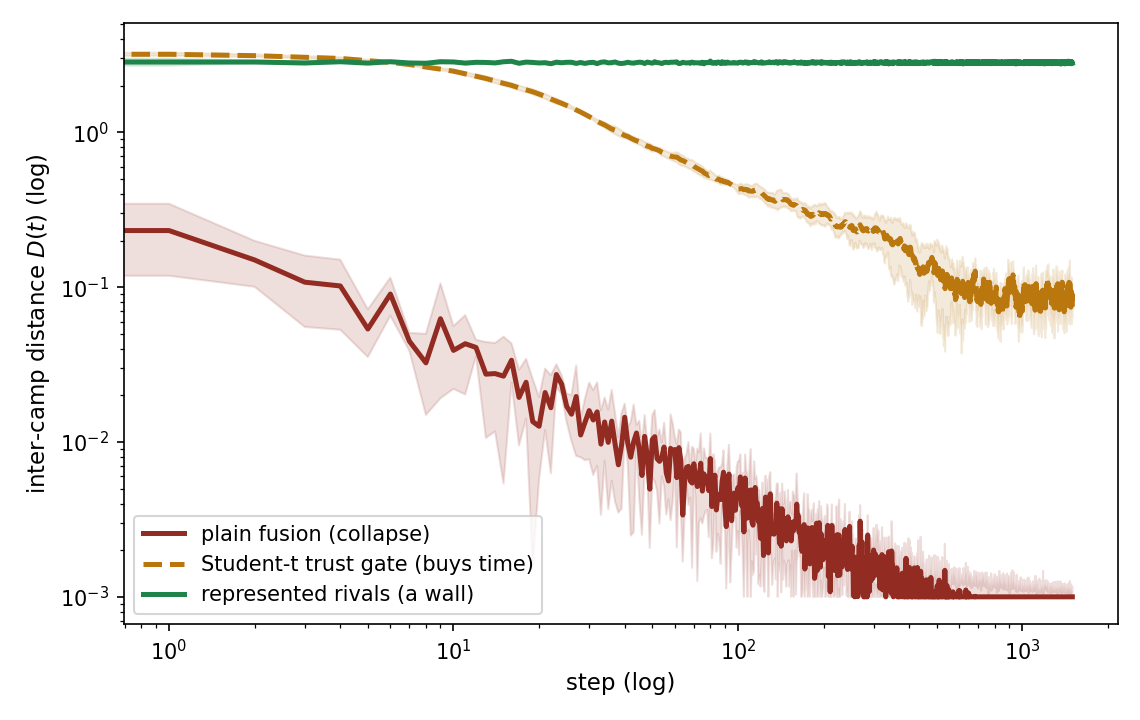
\includegraphics[width=0.7\linewidth]{fig_walls_vs_time.png}
\caption{Same setups, same evidence---only the representation differs (two camps, full
contact, theory-laden streams; inter-camp distance $D(t)$, mean $\pm$ s.d., 5 seeds, log--log).
Plain fusion collapses (the theorem); the Student-$t$ gate decays (time, bought and spent);
represented rivals hold (a wall). Each architecture runs its own best memory setting
(Appendix~\ref{app:reliability}).}
\label{fig:res-walls}
\end{figure}

Boundaries, stated plainly. The demonstrations are deliberately small---one agent, $N=60$,
then $N=16$, on hand-wired worlds---existence proofs that the wall was representational rather
than parametric, not sweeps of social topologies. The rival mechanism is \emph{given} its
candidates: the $K$ wirings are supplied, not discovered, and anchored forgetting on the
candidate nets is part of the mechanism---keeping a rival represented means not letting
accumulated evidence drown it (Appendix~\ref{app:reliability}). And what the mechanism does
not yet do is named, not hidden: under log-linear hypothesis pooling a lone discoverer's
candidate is majority-swamped---the discoverer problem returns one level up---and no agent yet
\emph{acts} on where its candidates disagree, the crucial experiment. Controls ship with each
experiment: a world that never shifts produces neither doubt nor variance inflation; gates and
rivals off reproduce the null regime byte-identically ($K=1$ is plain fusion); and no
acceptance bar is tuned anywhere (Appendix~\ref{app:reliability}).

% ======================================================================
\section{Discussion}
\label{sec:discussion}
% ======================================================================

Taken together, the results say the homogenization is a failure of \emph{representation}, not
of tuning---and each repair confirms the diagnosis by what it buys. Result 1 is the theorems
made visible: a community built from its field's default choices is the formalism's
\emph{normal-science} limit---smooth, cumulative refinement within a frame, consensus under
contact---and nothing in it entrenches, diverges, or breaks. Result 2 shows the wall stands
exactly where the theorems put it: make reliability a latent and an agent can at last be
surprised into doubt, a community can at last hold two wirings under contact---yet consensus
remains the only fixed point, so every protection the gate wins is a clock; represent the
rival itself and a wall finally stands. The characterization is of a stylized object---the
nets are hand-wired, the dials swept rather than inferred from data. What paradigm dynamics
still require, the measurement locates precisely, and its two nearest requirements are two
readings of one word.

\paragraph{Value as precision.}
The conviction field enters the dynamics as a tilt of the potential $h$: it represents
\emph{wanting}, and it buys displacement, not defense (Appendix~\ref{app:null}). The dogmatism
Kuhn describes---a commitment that resists revision because much is staked on it---is a statement
about stiffness, and stiffness lives in $\Pi$: value would have to enter as precision, a
convinced agent depositing internal evidence on the commitment it rehearses. The prediction is
concrete: lock-in becomes a race between internal rehearsal and pooled external evidence, so the
isolation boundary of Fig.~\ref{fig:res-lockin} should move with rehearsal rate instead of
pinning to zero contact.

\paragraph{Trust as inferred precision---now measured, and bounded.}
Result 2 is the conflict-resolution literature's canonical repair \citep{ohagan2012}, run at
both levels of the model, and its verdict anchors the discussion. Within an agent it buys heavy
tails, rejection, and falling confidence under contradiction---crisis rendered as a posterior;
between agents it makes stable schools \emph{attainable} on a connected graph holding shared
data, the configuration fixed trust forbids. But everything it buys, it buys as \emph{time}:
the gate is memoryless, its weights stay strictly positive, and consensus remains the only
place the dynamics can rest. The protection paradigm dynamics still lack is not a slower clock.

\paragraph{The missing slot is representational---and fillable.}
There is no coordinate in $(\Pi,h)$ whose value can mean \emph{torn between two hypotheses}: a
Gaussian belief net stores one mean and one always-unimodal precision, conflict arrives as
growing confidence (the theorems of \S\ref{sec:results}), and fusion erases who disagreed about
what---sources are anonymous once averaged. This is impoverishment by representation, not by
parameters, which is why no dial of the sweep escaped it and why the gate could only slow it.
The rival layer of \S\ref{sec:rivals} is that diagnosis made executable, and the wall of
Fig.~\ref{fig:res-walls} is what filling the slot buys: \emph{(i)} multiple structural
hypotheses per agent---$q_i(x,m)$ over candidate wirings, so an agent can be genuinely torn;
\emph{(ii)} divergence as state---the gap between an agent's live candidates is a quantity it
can compute and, in principle, act on; \emph{(iii)} communication of hypotheses---parameter
fusion within frames, log-linear pooling of hypothesis weights between them, never averaging
across frames. What remains open is named, not hidden: under log-linear pooling a lone
discoverer's candidate is majority-swamped---the discoverer problem returns one level up---and
no agent yet \emph{chooses} the experiment on which its live candidates disagree most, the
crucial experiment. Gates buy time; represented rivals buy walls; the next step is an agent
that acts on its rivals.

The model's relation to Kuhn can now be stated without allegory. The regime \emph{holds} normal
science, with a hard core and protective belt that are derived rather than decreed
\citep{lakatos1970}. Of the revolutionary remainder, inferred reliability \emph{supplies} crisis
as suspended confidence (the interior variance maximum of \S\ref{sec:res-distinct}) and renders
incommensurability \citep{kuhn1983} a timescale---a property of two histories' accumulated
confidence, not of two ideas. With rivals represented, incommensurability becomes a
\emph{state}: two camps internally certain of different wirings at a fixed point, not a
failure to converge---and the gestalt switch acquires its slot, a $q(m)$ that flips between
represented wirings when the prequential evidence turns. And one piece comes back as protocol
rather than representation: the fusion that crushes a staggered discovery vanishes when agents
abstain on dimensions they do not represent (Appendix~\ref{app:null})---real communities sit
somewhere between absence-as-denial and full abstention, an empirical question the model
converts from a confession into a measurement.

Any epistemic community whose aggregation step averages rather than gates inherits the regime's
signature, whatever the sophistication of its members. Aggregation by consensus-trained models is
precision-weighted pooling at scale: to the extent that machine-mediated science inserts such
aggregators into its loop, it will refine frames and never grow one. The model makes this
testable; it does not yet establish it. The same statement is a foundation for multi-agent active
inference at large: a population of structure learners is only as \emph{open-ended} as its
pooling permits---and as what its pooling \emph{reads}: a gate on opinions preserved nothing of
a pluralism that lived in wiring (\S\ref{sec:res-distinct}). Open-endedness is a property of the
protocol, to be designed in---not an emergent grace of scale.

The deepest exit lies beyond the present model class. Everything revolutionary above passes
through model expansion, and every candidate edits the prior over a fixed likelihood---while a
genuinely new \emph{instrument} enlarges the likelihood's own support. Structure learning over
latent structure is closed-loop; structure learning over the sensorium is not, and we know of no
agnostic stand-in for it as clean as the Poisson rate was for unconceived latents. This is the
formal face of the limit Stanford named: one cannot place a posterior over the unconceived
\citep{stanford2006}, only over whether one's model has missed something---enough to set how hard
an agent looks, never where (Appendix~\ref{app:closing}). What a community controls is how hard
it looks---and, these results say above all, what its pooling does to the member who finds it
first.

% ======================================================================
\begin{thebibliography}{99}

\bibitem[Albarracin et al.(2022)]{albarracin2022}
M.~Albarracin, D.~Demekas, M.~J.~D.~Ramstead, and C.~Heins.
Epistemic communities under active inference. \emph{Entropy}, 24(4):476, 2022.

\bibitem[\c{C}atal et al.(2024)]{catal2024}
O.~\c{C}atal, T.~Van~de~Maele, R.~J.~Pitliya, M.~Albarracin, C.~Pattisapu, and T.~Verbelen.
Belief sharing: a blessing or a curse. arXiv:2407.02465, 2024.

\bibitem[Dalege et al.(2016)]{dalege2016}
J.~Dalege, D.~Borsboom, F.~van Harreveld, H.~van den Berg, M.~Conner, and H.~L.~J.~van der Maas.
Toward a formalized account of attitudes: the Causal Attitude Network (CAN) model.
\emph{Psychological Review}, 123(1):2--22, 2016.

\bibitem[Dawid(1973)]{dawid1973}
A.~P.~Dawid.
Posterior expectations for large observations. \emph{Biometrika}, 60(3):664--667, 1973.

\bibitem[O'Hagan(1979)]{ohagan1979}
A.~O'Hagan.
On outlier rejection phenomena in Bayes inference.
\emph{Journal of the Royal Statistical Society, Series B}, 41(3):358--367, 1979.

\bibitem[O'Hagan and Pericchi(2012)]{ohagan2012}
A.~O'Hagan and L.~Pericchi.
Bayesian heavy-tailed models and conflict resolution: a review.
\emph{Brazilian Journal of Probability and Statistics}, 26(4):372--401, 2012.

\bibitem[Friedman et al.(2008)]{friedman2008glasso}
J.~Friedman, T.~Hastie, and R.~Tibshirani.
Sparse inverse covariance estimation with the graphical lasso.
\emph{Biostatistics}, 9(3):432--441, 2008.

\bibitem[Friston and Penny(2011)]{friston2011}
K.~J.~Friston and W.~Penny.
Post hoc Bayesian model selection. \emph{NeuroImage}, 56(4):2089--2099, 2011.

\bibitem[Friston et al.(2015)]{friston2015}
K.~Friston, F.~Rigoli, D.~Ognibene, C.~Mathys, T.~Fitzgerald, and G.~Pezzulo.
Active inference and epistemic value. \emph{Cognitive Neuroscience}, 6(4):187--214, 2015.

\bibitem[Friston et al.(2017)]{friston2017curiosity}
K.~J.~Friston, M.~Lin, C.~D.~Frith, G.~Pezzulo, J.~A.~Hobson, and S.~Ondobaka.
Active inference, curiosity and insight. \emph{Neural Computation}, 29(10):2633--2683, 2017.

\bibitem[Friston et al.(2018)]{friston2018bmr}
K.~J.~Friston, T.~Parr, and P.~Zeidman.
Bayesian model reduction. arXiv:1805.07092, 2018.

\bibitem[Hawkes(1971)]{hawkes1971}
A.~G.~Hawkes.
Spectra of some self-exciting and mutually exciting point processes.
\emph{Biometrika}, 58(1):83--90, 1971.

\bibitem[Hohwy(2016)]{hohwy2016}
J.~Hohwy.
The self-evidencing brain. \emph{No\^us}, 50(2):259--285, 2016.

\bibitem[Hughes et al.(2024)]{hughes2024}
E.~Hughes, M.~Dennis, J.~Parker-Holder, F.~Behbahani, A.~Mavalankar, Y.~Shi, T.~Schaul, and
T.~Rockt\"aschel.
Position: open-endedness is essential for artificial superhuman intelligence.
In \emph{Proceedings of the 41st International Conference on Machine Learning}, PMLR 235, 2024.

\bibitem[Hyland and Albarracin(2025)]{hyland2025}
D.~Hyland and M.~Albarracin.
On the variational costs of changing our minds. arXiv:2509.17957, 2025.
(Also in \emph{Active Inference: IWAI 2025}, CCIS vol.~2857, Springer, 2026,
doi:10.1007/978-3-032-16955-6\_1.)

\bibitem[Jonard et al.(2025)]{jonard2025}
N.~Jonard, S.~Reijula, and L.~Marengo.
Theory choice in epistemic networks: five ways to avoid premature convergence. PhilSci Archive, 2025.

\bibitem[Kitcher(1990)]{kitcher1990}
P.~Kitcher.
The division of cognitive labor. \emph{Journal of Philosophy}, 87(1):5--22, 1990.

\bibitem[Koller and Friedman(2009)]{koller2009}
D.~Koller and N.~Friedman.
\emph{Probabilistic Graphical Models: Principles and Techniques}. MIT Press, 2009.

\bibitem[Kuhn(1962)]{kuhn1962}
T.~S.~Kuhn.
\emph{The Structure of Scientific Revolutions}. University of Chicago Press, 1962.

\bibitem[MacKay(1992)]{mackay1992}
D.~J.~C.~MacKay.
Bayesian interpolation. \emph{Neural Computation}, 4(3):415--447, 1992.

\bibitem[Millidge et al.(2021)]{millidge2021}
B.~Millidge, A.~Tschantz, and C.~L.~Buckley.
Whence the expected free energy? \emph{Neural Computation}, 33(2):447--482, 2021.

\bibitem[Neal(1996)]{neal1996}
R.~M.~Neal.
\emph{Bayesian Learning for Neural Networks}.
Lecture Notes in Statistics 118, Springer, 1996.

\bibitem[Nguyen(2020)]{nguyen2018}
C.~T.~Nguyen.
Echo chambers and epistemic bubbles. \emph{Episteme}, 17(2):141--161, 2020.

\bibitem[O'Connor and Weatherall(2019)]{oconnor2019}
C.~O'Connor and J.~O.~Weatherall.
\emph{The Misinformation Age}. Yale University Press, 2019.

\bibitem[Parr and Friston(2017)]{parr2017uncertainty}
T.~Parr and K.~J.~Friston.
Uncertainty, epistemics and active inference.
\emph{Journal of the Royal Society Interface}, 14(136):20170376, 2017.

\bibitem[Smith et al.(2020)]{smith2020structure}
R.~Smith, P.~Schwartenbeck, T.~Parr, and K.~J.~Friston.
An active inference approach to modeling structure learning: concept learning as an example case.
\emph{Frontiers in Computational Neuroscience}, 14:41, 2020.

\bibitem[Stanford(2006)]{stanford2006}
P.~K.~Stanford.
\emph{Exceeding Our Grasp: Science, History, and the Problem of Unconceived Alternatives}.
Oxford University Press, 2006.

\bibitem[Stanley et al.(2017)]{stanley2017oe}
K.~O.~Stanley, J.~Lehman, and L.~Soros.
Open-endedness: the last grand challenge you've never heard of. \emph{O'Reilly Radar}, 2017.

\bibitem[Strevens(2003)]{strevens2003}
M.~Strevens.
The role of the priority rule in science. \emph{Journal of Philosophy}, 100(2):55--79, 2003.

\bibitem[Thagard(1989)]{thagard1989}
P.~Thagard.
Explanatory coherence. \emph{Behavioral and Brain Sciences}, 12(3):435--467, 1989.

\bibitem[Tipping(2001)]{tipping2001}
M.~E.~Tipping.
Sparse Bayesian learning and the relevance vector machine.
\emph{Journal of Machine Learning Research}, 1:211--244, 2001.

\bibitem[Zollman(2010)]{zollman2010}
K.~J.~S.~Zollman.
The epistemic benefit of transient diversity. \emph{Erkenntnis}, 72(1):17--35, 2010.

\bibitem[Griffiths and Ghahramani(2011)]{griffiths2011ibp}
T.~L.~Griffiths and Z.~Ghahramani.
The Indian Buffet Process: an introduction and review.
\emph{Journal of Machine Learning Research}, 12:1185--1224, 2011.

\bibitem[Kemp and Tenenbaum(2008)]{kemp2008form}
C.~Kemp and J.~B.~Tenenbaum.
The discovery of structural form.
\emph{Proceedings of the National Academy of Sciences}, 105(31):10687--10692, 2008.

\bibitem[Ullman et al.(2012)]{ullman2012}
T.~D.~Ullman, N.~D.~Goodman, and J.~B.~Tenenbaum.
Theory learning as stochastic search in a language of thought.
\emph{Cognitive Development}, 27(4):455--480, 2012.

\bibitem[Friston et al.(2017b)]{friston2017process}
K.~Friston, T.~FitzGerald, F.~Rigoli, P.~Schwartenbeck, and G.~Pezzulo.
Active inference: a process theory. \emph{Neural Computation}, 29(1):1--49, 2017.

\bibitem[Mathys et al.(2011)]{mathys2011}
C.~Mathys, J.~Daunizeau, K.~J.~Friston, and K.~E.~Stephan.
A Bayesian foundation for individual learning under uncertainty.
\emph{Frontiers in Human Neuroscience}, 5:39, 2011.

\bibitem[Smith et al.(2022)]{smith2022tutorial}
R.~Smith, K.~J.~Friston, and C.~Whyte.
A step-by-step tutorial on active inference and its application to empirical data.
\emph{Journal of Mathematical Psychology}, 107:102632, 2022.

\bibitem[Da Costa et al.(2020)]{dacosta2020}
L.~Da Costa, T.~Parr, N.~Sajid, S.~Veselic, V.~Neacsu, and K.~Friston.
Active inference on discrete state-spaces: a synthesis.
\emph{Journal of Mathematical Psychology}, 99:102447, 2020.

\bibitem[Holmes(2000)]{holmes2000}
F.~L.~Holmes.
The revolution in chemistry and physics: overthrow of a reigning paradigm or competition between
contemporary research programs? \emph{Isis}, 91(4):735--753, 2000.

\bibitem[Thagard(1990)]{thagard1990}
P.~Thagard.
The conceptual structure of the chemical revolution.
\emph{Philosophy of Science}, 57(2):183--209, 1990.

\bibitem[Boantza and Gal(2011)]{boantza2011}
V.~D.~Boantza and O.~Gal.
The `absolute existence' of phlogiston: the losing party's point of view.
\emph{British Journal for the History of Science}, 44(3):317--342, 2011.

\bibitem[Blumenthal and Ladyman(2017)]{blumenthal2017}
G.~Blumenthal and J.~Ladyman.
The development of problems within the phlogiston theories, 1766--1791.
\emph{Foundations of Chemistry}, 19(3):241--280, 2017.

\bibitem[Ball et al.(2024)]{polygraphs2024}
B.~Ball, A.~Koliousis, A.~Mohanan, and M.~Peacey.
Computational philosophy: reflections on the {PolyGraphs} project.
\emph{Humanities and Social Sciences Communications}, 11:186, 2024.

\bibitem[Michelini et al.(2023)]{michelini2023}
M.~Michelini, J.~Osorio, W.~Houkes, D.~\v{S}e\v{s}elja, and C.~Stra\ss{}er.
Scientific disagreements and the diagnosticity of evidence: how too much data may lead to polarization.
\emph{Journal of Artificial Societies and Social Simulation}, 26(4):5, 2023.

\bibitem[Albarracin et al.(2024)]{albarracin2024protentions}
M.~Albarracin, R.~J.~Pitliya, T.~St.~Clere Smithe, D.~A.~Friedman, K.~Friston, and M.~J.~D.~Ramstead.
Shared protentions in multi-agent active inference.
\emph{Entropy}, 26(4):303, 2024.

\bibitem[Friston et al.(2024a)]{friston2023federated}
K.~J.~Friston, T.~Parr, C.~Heins, A.~Constant, D.~Friedman, T.~Isomura, C.~Fields,
T.~Verbelen, M.~Ramstead, J.~Clippinger, and C.~D.~Frith.
Federated inference and belief sharing.
\emph{Neuroscience \& Biobehavioral Reviews}, 156:105500, 2024.

\bibitem[Waade et al.(2025)]{waade2025}
P.~T.~Waade, C.~L.~Olesen, J.~E.~Laursen, S.~W.~Nehrer, C.~Heins, K.~Friston, and C.~Mathys.
As one and many: relating individual and emergent group-level generative models in active inference.
\emph{Entropy}, 27(2):143, 2025.

\bibitem[Ullman and Tenenbaum(2020)]{ullman2020}
T.~D.~Ullman and J.~B.~Tenenbaum.
Bayesian models of conceptual development: learning as building models of the world.
\emph{Annual Review of Developmental Psychology}, 2:533--558, 2020.

\bibitem[Neacsu et al.(2022)]{neacsu2022}
V.~Neacsu, M.~B.~Mirza, R.~A.~Adams, and K.~J.~Friston.
Structure learning enhances concept formation in synthetic active inference agents.
\emph{PLOS ONE}, 17(11):e0277199, 2022.

\bibitem[Priorelli and Stoianov(2023)]{priorelli2023}
M.~Priorelli and I.~P.~Stoianov.
Dynamic inference by model reduction.
\emph{bioRxiv}, 2023. doi:10.1101/2023.09.10.557043.

\bibitem[Friston et al.(2016)]{friston2016peb}
K.~J.~Friston, V.~Litvak, A.~Oswal, A.~Razi, K.~E.~Stephan, B.~C.~M.~van Wijk, G.~Ziegler, and
P.~Zeidman. Bayesian model reduction and empirical {Bayes} for group ({DCM}) studies.
\emph{NeuroImage}, 128:413--431, 2016.

\bibitem[Friston et al.(2024b)]{friston2024ci}
K.~J.~Friston et al.
Designing ecosystems of intelligence from first principles.
\emph{Collective Intelligence}, 3(4), 2024. arXiv:2212.01354.

\bibitem[Kaufmann et al.(2021)]{kaufmann2021}
R.~Kaufmann, P.~Gupta, and J.~Taylor.
An active inference model of collective intelligence.
\emph{Entropy}, 23(7):830, 2021.

\bibitem[Acemoglu and Ozdaglar(2011)]{acemoglu2011}
D.~Acemoglu and A.~Ozdaglar.
Opinion dynamics and learning in social networks.
\emph{Dynamic Games and Applications}, 1(1):3--49, 2011.

\bibitem[Bala and Goyal(1998)]{balagoyal1998}
V.~Bala and S.~Goyal.
Learning from neighbours. \emph{Review of Economic Studies}, 65(3):595--621, 1998.

\bibitem[Bohren and Hauser(2021)]{bohren2021}
J.~A.~Bohren and D.~N.~Hauser.
Learning with heterogeneous misspecified models: characterization and robustness.
\emph{Econometrica}, 89(6):3025--3077, 2021.

\bibitem[Bollen(1987)]{bollen1987}
K.~A.~Bollen.
Total, direct, and indirect effects in structural equation models.
\emph{Sociological Methodology}, 17:37--69, 1987.

\bibitem[Bonacich(1987)]{bonacich1987}
P.~Bonacich.
Power and centrality: a family of measures.
\emph{American Journal of Sociology}, 92(5):1170--1182, 1987.

\bibitem[DeGroot(1974)]{degroot1974}
M.~H.~DeGroot.
Reaching a consensus. \emph{Journal of the American Statistical Association}, 69(345):118--121, 1974.

\bibitem[Feyerabend(1975)]{feyerabend1975}
P.~Feyerabend.
\emph{Against Method}. New Left Books, 1975.

\bibitem[Genest and Zidek(1986)]{genest1986}
C.~Genest and J.~V.~Zidek.
Combining probability distributions: a critique and an annotated bibliography.
\emph{Statistical Science}, 1(1):114--135, 1986.

\bibitem[Hegselmann and Krause(2002)]{hegselmann2002}
R.~Hegselmann and U.~Krause.
Opinion dynamics and bounded confidence: models, analysis and simulation.
\emph{Journal of Artificial Societies and Social Simulation}, 5(3), 2002.

\bibitem[Katz(1953)]{katz1953}
L.~Katz.
A new status index derived from sociometric analysis. \emph{Psychometrika}, 18(1):39--43, 1953.

\bibitem[Kuhn(1983)]{kuhn1983}
T.~S.~Kuhn.
Commensurability, comparability, communicability.
\emph{PSA: Proceedings of the Biennial Meeting of the Philosophy of Science Association},
1982(2):669--688, 1983.

\bibitem[Lakatos(1970)]{lakatos1970}
I.~Lakatos.
Falsification and the methodology of scientific research programmes.
In I.~Lakatos and A.~Musgrave, editors, \emph{Criticism and the Growth of Knowledge},
pages 91--196. Cambridge University Press, 1970.

\bibitem[Laudan(1977)]{laudan1977}
L.~Laudan.
\emph{Progress and Its Problems: Towards a Theory of Scientific Growth}.
University of California Press, 1977.

\bibitem[Laudan(1984)]{laudan1984}
L.~Laudan.
\emph{Science and Values: The Aims of Science and Their Role in Scientific Debate}.
University of California Press, 1984.

\bibitem[Lehrer and Wagner(1981)]{lehrer1981}
K.~Lehrer and C.~Wagner.
\emph{Rational Consensus in Science and Society}. D.~Reidel, 1981.

\bibitem[Malioutov et al.(2006)]{malioutov2006}
D.~M.~Malioutov, J.~K.~Johnson, and A.~S.~Willsky.
Walk-sums and belief propagation in Gaussian graphical models.
\emph{Journal of Machine Learning Research}, 7:2031--2064, 2006.

\bibitem[O'Connor and Weatherall(2018)]{oconnorpolar2018}
C.~O'Connor and J.~O.~Weatherall.
Scientific polarization. \emph{European Journal for Philosophy of Science}, 8(3):855--875, 2018.

\bibitem[Ortega and Braun(2013)]{ortega2013}
P.~A.~Ortega and D.~A.~Braun.
Thermodynamics as a theory of decision-making with information-processing costs.
\emph{Proceedings of the Royal Society A}, 469(2153):20120683, 2013.

\bibitem[Todorov(2009)]{todorov2009}
E.~Todorov.
Efficient computation of optimal actions.
\emph{Proceedings of the National Academy of Sciences}, 106(28):11478--11483, 2009.

\bibitem[Wright(1934)]{wright1934}
S.~Wright.
The method of path coefficients. \emph{Annals of Mathematical Statistics}, 5(3):161--215, 1934.

\bibitem[Zollman(2013)]{zollman2013}
K.~J.~S.~Zollman.
Network epistemology: communication in epistemic communities.
\emph{Philosophy Compass}, 8(1):15--27, 2013.

\end{thebibliography}

% ======================================================================
\clearpage
\appendix
% ======================================================================
\section{The operator, the tilt, and the Schur residue}
\label{app:operator}
% ======================================================================

\paragraph{Linear-Gaussian construction.} The couplings form a structural equation model $x=Ax+\zeta$,
$\zeta\sim\mathcal N(0,D^{-1})$ with $A$ the weighted DAG adjacency \citep{koller2009}; the choice is
for tractability, and a nonlinear coupling would replace $\Top$ by a local linearization. The
propagation operator is the resolvent
\begin{equation}
\Top=(I-A)^{-1}=\sum_{k\ge 0}A^k,\qquad
\Top_{iw}=\!\!\sum_{\text{paths }i\rw w}\ \prod \pi\ =\ \pi_{i\rw w},
\label{eq:Top-full}
\end{equation}
the Neumann series finite because a DAG makes $A$ nilpotent. We realise $\Top$ on the coupling
magnitudes $|A|$ so downstream mass does not cancel when a child opposes a parent; the signed $A$
builds the precision matrix. We index $\Top$ so that $\kappa_i$ sums row $i$; under the SEM
convention the released code stores the transpose and computes the same fields as column-sums of
$\Top^{\!\top}$, so a reader reproducing $\Top\bone$ literally against the code's array must
transpose first.

\paragraph{The value tilt.} With honest posterior $p(x\mid o,G)=\mathcal N(\mu,\Sigma)$, the tilted
posterior of Eq.~\eqref{eq:tilted} is a pure mean shift,
$q_\lambda(x)=\mathcal N(\mu+\lambda\Sigma U,\,\Sigma)$, with cumulant-generating function
$Z(\lambda)=\lambda\,U^{\!\top}\!\mu+\tfrac12\lambda^2\,U^{\!\top}\!\Sigma U$. Note that gating a
channel ($\rho_k\to0$) \emph{raises} the posterior variance and hence $Z''$; lock-in lives in the
vanishing mean-update gain $\rho_k H_k\Sigma U$, not in the curvature.

The mind-change cost of Eq.~\eqref{eq:tilted} is anchored to the network prior
$p(x\mid G)=\mathcal N(\mu_0,\Pi_0^{-1})$: the revision $q_\lambda$ pays
\begin{equation}
\KL{q_\lambda}{p(x\mid G)}
=\tfrac12\,\delta^{\!\top}\Pi_0\,\delta
+\tfrac12\bigl[\operatorname{tr}(\Pi_0\Sigma)-\log\det(\Pi_0\Sigma)-d\bigr],
\label{eq:mindcost}
\end{equation}
with $\delta=\mu+\lambda\Sigma U-\mu_0$ and $d=\dim x$: the evidence-driven and value-driven
displacements are priced \emph{together}, in
the prior precision $\Pi_0$---exactly the off-diagonal mass the carry-over field $\kappa=\Top\bone$
summarizes. The smaller quantity $\KL{q_\lambda}{p(x\mid o,G)}=\tfrac12\lambda^2\,U^{\!\top}\!\Sigma U$
is the fidelity gap to the honest posterior, not the cost of changing one's mind: it would vanish
for an agent that followed the evidence exactly, however far the evidence moved it.

\begin{figure}[h!]
\centering
\begin{subfigure}{0.49\textwidth}\centering
\resizebox{0.92\linewidth}{!}{%
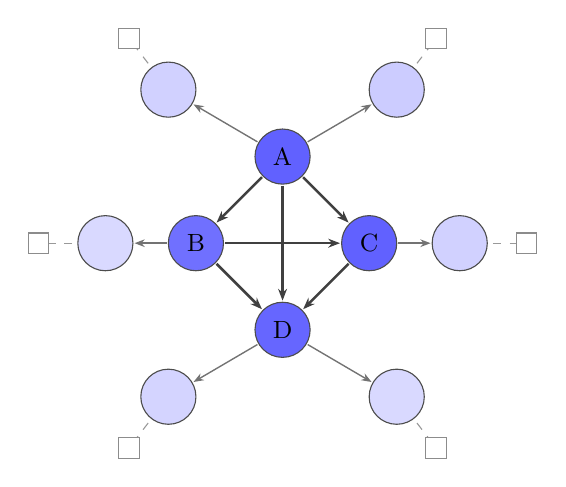
\begin{tikzpicture}
  \Positions \Edges
  \node[bel,fill=blue!62!white] at (A){A};
  \node[bel,fill=blue!56!white] at (B){B};
  \node[bel,fill=blue!62!white] at (C){C};
  \node[bel,fill=blue!60!white] at (D){D};
  \node[bel,fill=blue!18!white] at (b1){};
  \node[bel,fill=blue!20!white] at (b2){};
  \node[bel,fill=blue!15!white] at (b3){};
  \node[bel,fill=blue!18!white] at (b4){};
  \node[bel,fill=blue!17!white] at (b5){};
  \node[bel,fill=blue!15!white] at (b6){};
\end{tikzpicture}}
\par\vspace{4pt}
\resizebox{0.74\linewidth}{!}{%
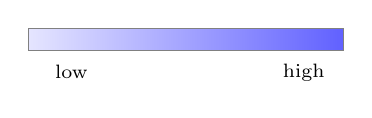
\begin{tikzpicture}
  \shade[left color=blue!10!white,right color=blue!62!white] (0,0) rectangle (4,0.28);
  \draw[black!50,line width=0.3pt] (0,0) rectangle (4,0.28);
  \node[font=\scriptsize] at (0.55,-0.28){low}; \node[font=\scriptsize] at (3.5,-0.28){high};
\end{tikzpicture}}
\caption{Revision cost $\kappa_i$ (conservatism)}
\label{sub:cost}
\end{subfigure}
\hfill
\begin{subfigure}{0.49\textwidth}\centering
\resizebox{0.92\linewidth}{!}{%
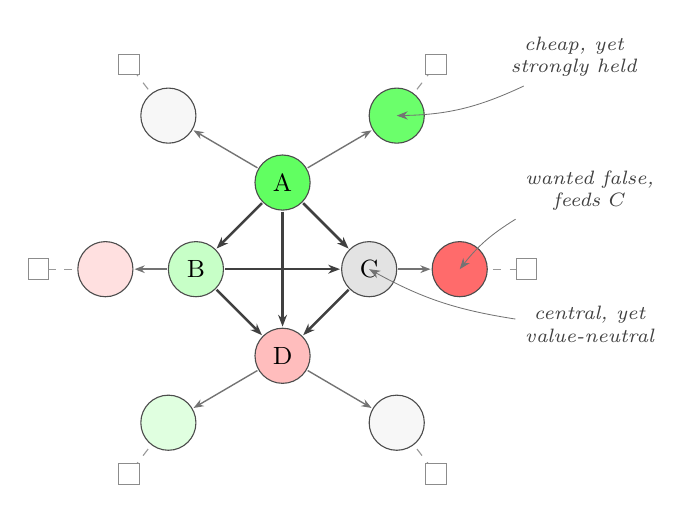
\begin{tikzpicture}
  \Positions \Edges
  \node[bel,fill=green!62!white] at (A){A};
  \node[bel,fill=green!22!white] at (B){B};
  \node[bel,fill=gray!22!white]  at (C){C};
  \node[bel,fill=red!26!white]   at (D){D};
  \node[bel,fill=gray!6!white]   at (b1){};
  \node[bel,fill=green!58!white] at (b2){};
  \node[bel,fill=red!12!white]   at (b3){};
  \node[bel,fill=red!58!white]   at (b4){};
  \node[bel,fill=green!12!white] at (b5){};
  \node[bel,fill=gray!6!white]   at (b6){};
  \node[anno] (an2) at (3.7,2.7){cheap, yet\\strongly held};
  \draw[annoarrow] (an2) to[bend left=12] (b2);
  \node[anno] (anC) at (3.9,-0.7){central, yet\\value-neutral};
  \draw[annoarrow] (anC) to[bend left=10] (C);
  \node[anno] (an4) at (3.9,1.0){wanted false,\\feeds $C$};
  \draw[annoarrow] (an4) to[bend right=10] (b4);
\end{tikzpicture}}
\par\vspace{4pt}
\resizebox{0.88\linewidth}{!}{%
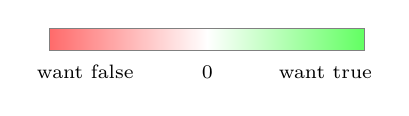
\begin{tikzpicture}
  \shade[left color=red!58!white,right color=white] (0,0) rectangle (2,0.28);
  \shade[left color=white,right color=green!62!white] (2,0) rectangle (4,0.28);
  \draw[black!50,line width=0.3pt] (0,0) rectangle (4,0.28);
  \node[font=\scriptsize] at (0.45,-0.28){want false}; \node[font=\scriptsize] at (2,-0.28){0};
  \node[font=\scriptsize] at (3.5,-0.28){want true};
\end{tikzpicture}}
\caption{Intrinsic utility $u_i$ (conviction)}
\label{sub:util}
\end{subfigure}
\caption{Two fields on one paradigm (schematic). Both panels carry the \emph{same} network---a densely
coupled core $\{A,B,C,D\}$ and a sparse belt $\{b_1,\dots,b_6\}$ in contact with observation.
\subref{sub:cost}~Revision cost is the carry-over of mind-change, $\kappa=\Top\bone$
(Eq.~\ref{eq:kappa}): a node's cost is the precision-weighted mass of its descendants, a clean radial
gradient monotone in centrality. \subref{sub:util}~Intrinsic utility is signed---beliefs one wants
true (green), wants false (red), or is neutral toward (white)---and the conviction field
$U=\Top u$ does not align with $\kappa$: $C$ is central yet value-neutral; $b_2$ is cheap yet strongly
held; $b_4$, which feeds $C$, is a conclusion the community wants false. The two fields are
$\Top\bone$ and $\Top u$, the same operator on two sources, and they are independent vectors.}
\label{fig:twofields}
\end{figure}

\paragraph{The Schur residue.} Marginalizing a hub condenses its influence into new edges among its
neighbours: for a common-cause structure over $(x_1,x_2,b)$,
\begin{equation}
\Pi=\begin{pmatrix}2&0&1\\0&2&1\\1&1&2\end{pmatrix}
\ \xrightarrow{\ \text{marginalize } b\ }\
\begin{pmatrix}2&0\\0&2\end{pmatrix}-\tfrac12\begin{pmatrix}1\\1\end{pmatrix}\begin{pmatrix}1&1\end{pmatrix}
=\begin{pmatrix}1.5&-0.5\\-0.5&1.5\end{pmatrix},
\label{eq:schur}
\end{equation}
a direct coupling induced where the joint had a zero. Conditioning on a shared \emph{effect} is the
dual operation: two commitments that jointly feed one observation are a priori independent, and
clamping that observation anti-couples them---explaining away, run on the precision matrix. Both
operations fill in the off-diagonal coupling the carry-over cost is built from, and
Fig.~\ref{fig:schur-generic} draws both on the smallest nets that exhibit them.

\begin{figure}[h!]
\centering
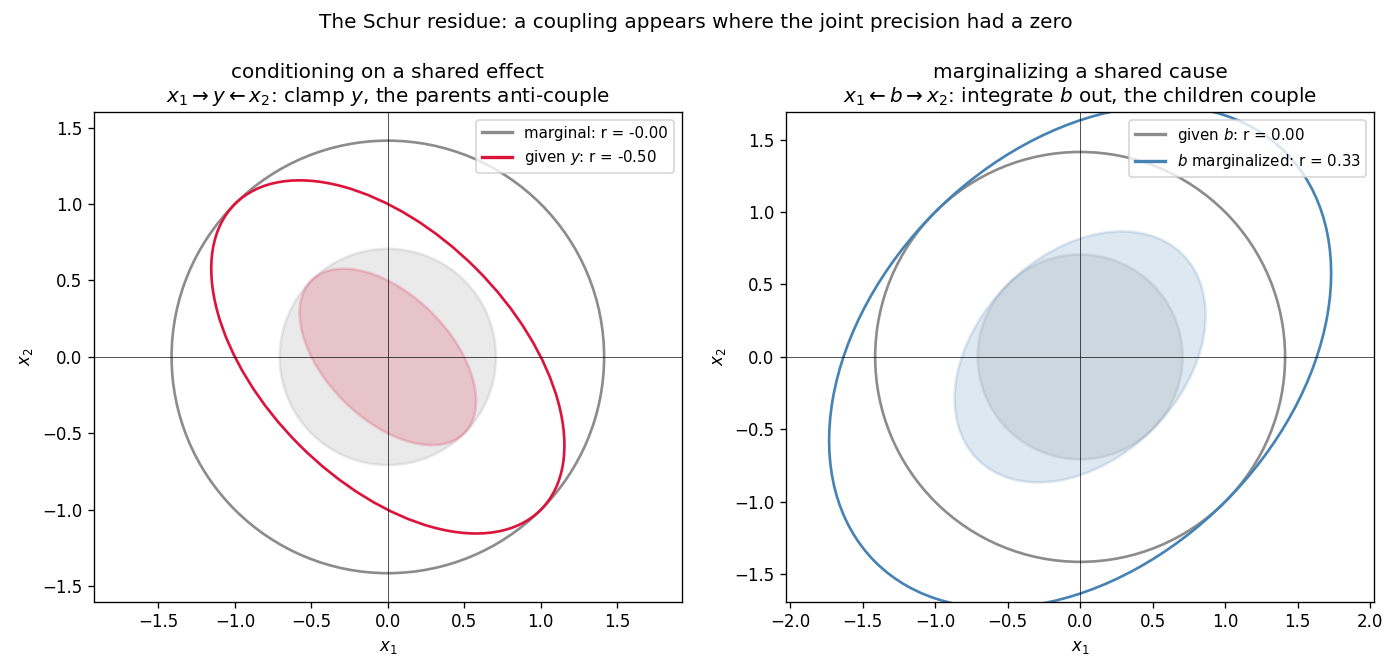
\includegraphics[width=\linewidth]{fig_schur_generic.png}
\caption{The Schur residue, computed on the smallest nets that show it. \emph{Left:} conditioning
on a shared effect ($x_1\!\to\!y\!\leftarrow\!x_2$): the parents are a priori independent (grey,
$r=0$); clamping their common descendant $y$ manufactures an anti-correlation (crimson,
$r=-0.50$)---explaining away. \emph{Right:} marginalizing a shared cause (the matrix of
Eq.~\ref{eq:schur}): the children are independent given $b$ (grey); integrating $b$ out leaves
them coupled (blue, $r=+0.33$). In both cases a coupling appears where the joint precision had a
zero---the off-diagonal mass the carry-over cost $\kappa=\Top\bone$ is built from.}
\label{fig:schur-generic}
\end{figure}

% ======================================================================
\section{The null regime, measured}
\label{app:null}
% ======================================================================

This appendix carries the quantitative characterization of the default (fixed-reliability)
community summarized in \S\ref{sec:res-homogeneity}: the full Kuhnian-cycle sweep on the
phlogiston world---normal science, the gravimetric anomaly, crisis, reduction, discovery of
oxygen, every phase a threshold crossing of the agents' own evidence, none stipulated---over
the dials of Table~\ref{tab:dials}, spanning the baseline and every mechanism of
Appendix~\ref{app:closing}.

\begin{table}[h!]
\centering\footnotesize
\begin{tabular}{lll}
\hline
Dial & Symbol & What it controls \\
\hline
Social coupling & \emph{inter} & inter-community trust weight (0 = isolation) \\
Vanguard fraction & --- & fraction of agents in the open (low-$\lambda$) community \\
Conviction & $\lambda_d$ & dogmatic community's value tilt / prune protection \\
Gate scaling & $s$ & strength of the conviction gate on disconfirming channels \\
Proposal rate & $r$ (Poisson) & arrival rate of structural proposals \\
Forgetting & $\omega\in(0,1]$ & decay of accumulated evidence toward the prior \\
Observation noise & $\sigma_o$ & sensory noise at the belt \\
Channel reliability & $\nu$ & Student-$t$ gate on the agent's own channels (off $=$ Gaussian) \\
Social trust & $\nu_s$ & Student-$t$ gate on the fusion weights (off $=$ fixed trust) \\
Fusion protocol & --- & pool all dimensions (delta) vs.\ jointly represented (abstention) \\
Closed-loop mechanisms & $\beta,\tau,\kappa_r,\lambda_c,\epsilon$ & adequacy-driven rate, social
excitation, audit credit, value accretion (Appendix~\ref{app:closing}) \\
\hline
\end{tabular}
\caption{The dials swept in the experiments; all other quantities are held fixed. The last two
rows are protocol and mechanism variations layered on the baseline; each defaults to ``off''
(constant rate, one-shot accept, delta pooling, static $u$, both reliability gates off),
reproducing the baseline model exactly.}
\label{tab:dials}
\end{table}

\paragraph{Only total isolation protects a superseded paradigm.}
The setup pits a dogmatic community---high conviction, whose agents gate their own disconfirming
channels (\S\ref{sec:revision})---against an open vanguard already tracking the anomaly, and
dials the inter-community trust weight \emph{inter} from $0$ (sealed off) to dense contact.
Sealed off, the gating protects: under strong gating ($s=10$) only $19\%$ ever convert. But at
\emph{inter}$=0.005$, $92\%$ convert to oxygen, however strong the gate and however dogmatic the
agents, and the transition is a sharp boundary, not a gradual fade (Fig.~\ref{fig:res-lockin}).
A control pins down what does the stalling: keep conviction exactly as high but switch the
self-gating off, and the community revolts in full (revolted fraction $1.0$ versus $0.0$,
$\gamma\to1$). The tilt never stalls anyone (Eq.~\ref{eq:gamma}); its one causal route to
lock-in runs through the gate, and the gate loses to the faintest connection, because a
neighbour's evidence arrives weighted by trust, not by the receiver's conviction. Motivated
reasoning in this regime is \emph{wishful}, not \emph{dogmatic}: a bias lives in the potential
$h$; an entrenchment would have to live in the precision $\Pi$---which is exactly where the
inferred-reliability gate of \S\ref{sec:reliability} puts it.

\begin{figure}[h!]
\centering
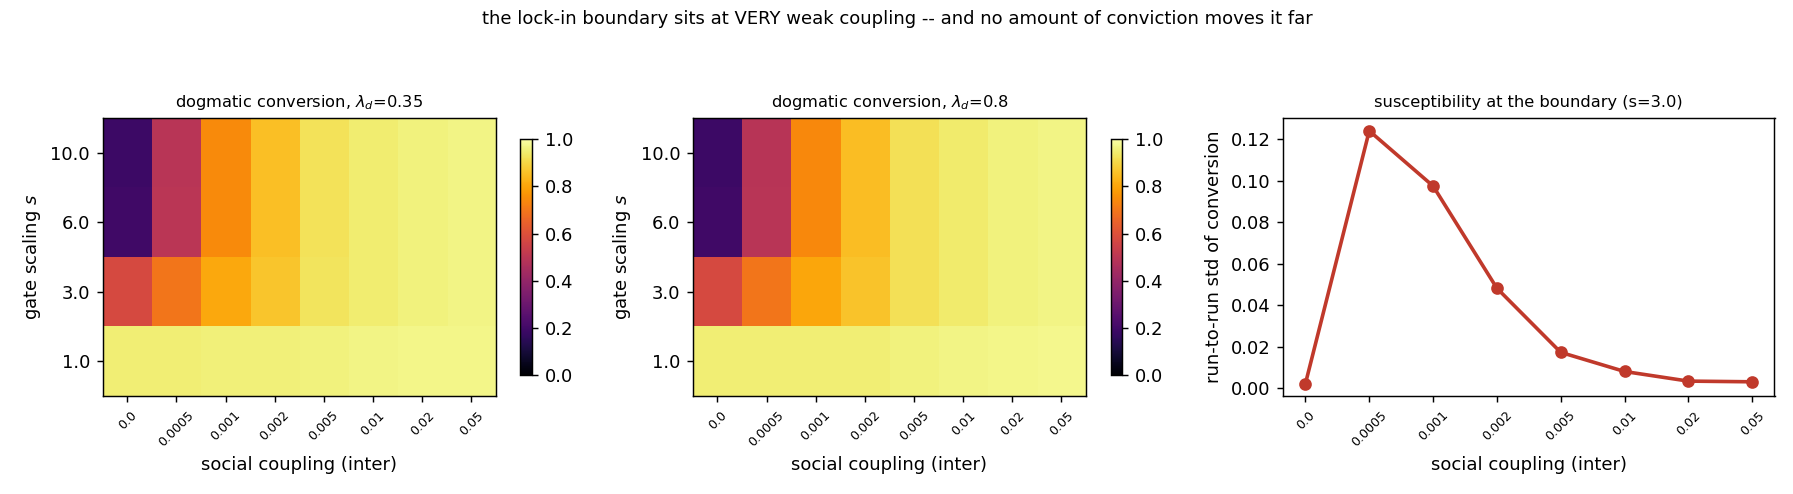
\includegraphics[width=\linewidth]{fig_kuhn_lockin_boundary.png}
\caption{Only isolation protects a superseded paradigm (phlogiston sweep, fixed trust).
\emph{Left, centre:} the fraction of the dogmatic community that converts to oxygen, as a
function of contact (\emph{inter}) and of how strongly conviction gates disconfirming channels
($s$), at two conviction levels ($\lambda_d=0.35$ and $0.8$). Past
\emph{inter}$\,\approx0.005$ nearly everyone converts, and doubling conviction barely changes
the picture. \emph{Right:} the run-to-run spread spikes in a narrow band around
\emph{inter}$\,\approx5\times10^{-4}$: a sharp boundary, not a fade.}
\label{fig:res-lockin}
\end{figure}

\paragraph{Pooling kills the lone discoverer---by protocol, not by principle.}
Discovery means waking a node---oxygen---that no agent's network yet contains; candidates arrive
at random (Poisson rate $r$, \S\ref{sec:structurelearning}), and the fraction that discovers
follows the waiting-time law $1-(1-r)^T$. What the rate governs is survival: under the baseline
fusion, a discovery made by one agent at a time is averaged away every time, because delta
pooling reads \emph{has no such variable}---a fact about an agent's model class---as
\emph{maximally certain it is zero}, a belief within its support
\citep{genest1986,friston2023federated}. The corrected protocol is dimension-aware
\emph{abstention} pooling: each entry of the precision matrix is pooled only over the neighbours
that represent it. The consequence is a wholesale relocation of the survival threshold
(Fig.~\ref{fig:res-fusion}): under delta pooling staggered survival is zero at every rate; under
abstention pooling it tracks the discovery fraction itself ($0.39/0.64/0.86$ at
$r_0=0.005/0.01/0.02$).

\begin{figure}[h!]
\centering
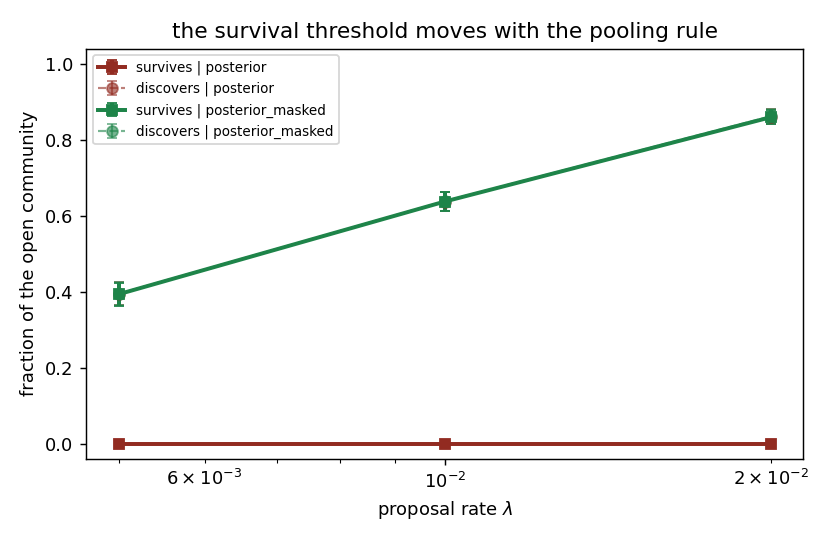
\includegraphics[width=0.62\linewidth]{fig_kuhn_fusion.png}
\caption{The survival threshold moves with the pooling protocol (32 seeds per cell). Solid:
fraction of the open community whose concept survives; dashed: fraction that discovers at all.
Under delta pooling (red) a pinned slot is a confident ``no such thing'' and staggered survival
is zero at every rate; under abstention pooling (green) survival tracks discovery.
Incommensurability as a population-level force is a property of the protocol, not of the
concepts.}
\label{fig:res-fusion}
\end{figure}

\paragraph{Every escape goes around the averaging, never through it.}
The sweep's remaining mechanisms sharpen the same conclusion (Table~\ref{tab:escapes}; full
results in Appendix~\ref{app:closing}). None of them lets two connected communities holding the
same data \emph{remain} in disagreement: each either re-times the passage through the consensus
bottleneck or synchronizes the population for it.

\begin{table}[h!]
\centering\footnotesize
\begin{tabular}{p{0.20\linewidth}p{0.24\linewidth}p{0.30\linewidth}p{0.16\linewidth}}
\hline
Escape & What it changes & Measured effect & Verdict \\
\hline
Adequacy-inferred rate & \emph{when} the community looks & crisis-to-discovery $55\to29$ steps;
matched by a constant rate of equal mean & re-times the passage \\[2pt]
Social excitation (Hawkes) & how nearly \emph{together} it looks & waking dispersion $64\to2$
steps; staggered survival $0\to0.88$--$0.95$ & synchrony outruns the averaging \\[2pt]
Audited wake-then-prune & whether curiosity is \emph{safe} & null world: $100\%$ of wakes
re-pinned, exactly & keeps the search honest \\[2pt]
Value accretion & conviction grown from \emph{inside} & conversion delayed $\sim2.2\times$, never
prevented & buys time, not immunity \\
\hline
\end{tabular}
\caption{Four mechanisms layered on the fixed-reliability baseline, none of which opens the
consensus engine (Appendix~\ref{app:closing}).}
\label{tab:escapes}
\end{table}

\paragraph{Robustness.}
The arc is robust across forgetting and observation noise ($\omega\in[0.9,1.0]$,
$\sigma_o\in[0.25,1.0]$): crisis and reduction survive everywhere---including the no-forgetting
wall $\omega=1$, where only discovery thins: a community that never forgets still sees its
paradigm die, but loses the capacity to grow the successor. Each experiment ships its own null
and positive controls---a world that never shifts produces neither crisis nor discovery; the
gated, isolated community stays locked; Poisson discovery follows the waiting-time law---and no
acceptance bar is tuned anywhere: the wake's sole accept test is the model log Bayes factor
(Appendix~\ref{app:crisis-discovery}); whatever the derivations there do not fix is named there
as a commitment.

% ======================================================================
\section{Inferred reliability and represented rivals: definitions and experiment details}
\label{app:reliability}
% ======================================================================

\paragraph{The three reads of one functional.}
Every gate in the paper is the Student-$t$ scale-mixture weight
$\eta=(\nu+1)/(\nu+z^2)$---the posterior expectation of a source's latent noise scale given
its standardized squared surprise $z^2$ (one E-step of the EM view of $t$-regression)---applied
to three different surprises. \emph{Channels:} $z_k^2=(o_k-(H\mu)_k)^2/\mathrm{predvar}_k$ with
$\mathrm{predvar}_k=\sigma_o^2+(H\Pi^{-1}H^{\!\top})_{kk}$, the agent's own surprise at
observation $k$ before depositing it; $\eta_k$ multiplies the channel's deposit, composing
with the conviction gate of \S\ref{sec:revision}. \emph{Opinions:}
$z_{ij}^2=\sum_v(\mu_j[v]-\mu_i[v])^2/(\Pi_i[v,v]^{-1}+\Pi_j[v,v]^{-1})$, the calibrated
disagreement of two posteriors summed over the measured nodes (summed, not averaged: a localized
heresy must be able to sever trust); $\eta_{ij}$ multiplies the fusion weights, whose row
normalization absorbs the overall scale. \emph{Wiring:} the same sum taken over contested
coupling entries $x=\Pi[a,c]$, normalized by their pairwise symmetric scale
$\max((x_i^2+x_j^2)/2,\,\epsilon^2)$---bounded per coupling, and invariant to the global
precision growth the forgetting equilibrium produces, so it reads \emph{how} two agents wire
the world, not how much evidence they hold.

\paragraph{Represented rivals: definitions.}
Each agent carries $K$ candidate nets $(\Pi_{ik},h_{ik})$ and log-weights $L_{ik}$ over a
model index. Per step, every candidate is scored by its prequential predictive density
\emph{before} the shared deposit lands, $\log p(o_t\mid o_{<t},M_k)$, so
structure-discriminating evidence accumulates in $L$ rather than being erased by the Fisher
deposit (which never sees the observation's value). Fusion is hypothesis-aligned---candidate
$k$ pools only with neighbours' candidate $k$---and the log-weights pool log-linearly with
damping $\alpha_m$: $L\leftarrow(1-\alpha_m)L+\alpha_m WL$. Deviations of the pooled log-odds
from the population mean converge to $(I-W)^{+}(s-\bar s)/\alpha_m$, a constant gap of
${\sim}\,s/2\alpha_m$ nats for two symmetric camps: a genuine fixed point---the wall of
Fig.~\ref{fig:res-walls}---whose height the early-measured per-step source predicts
conservatively (realized $110$ nats at the horizon, tail still growing at $+0.016$ nats/step).
Anchored forgetting on the candidate nets,
$\Pi_{ik}\leftarrow\Pi_{0k}+\omega(\Pi_{ik}-\Pi_{0k})$, is part of the mechanism: without it
every candidate's precision grows without bound and their predictive densities converge. $K=1$
reduces exactly to plain fuse-then-observe, which is how the Gaussian baselines run on
byte-identical observation streams; each architecture runs its own best memory setting.

\paragraph{The experiments.}
Table~\ref{tab:rel-experiments} lists the gated configurations; all are seeded,
assertion-checked at run time, and write their summary statistics next to their figures. The
rows below the rule are population-level runs of the same gates through the full Kuhnian
cycle---denial and rehabilitation of doubted channels, schism thresholds in accumulated
confidence, self-organized and then self-undone isolation---reported here rather than in the
main text because each is a further reading of the same two results: homogenization delayed,
never escaped.

\begin{table}[h!]
\centering\footnotesize
\begin{tabular}{p{0.23\linewidth}p{0.36\linewidth}p{0.32\linewidth}}
\hline
Experiment & Setup & Headline \\
\hline
Conflict crisis (\S\ref{sec:res-distinct}) & 1 agent, chain $A{\to}B{\to}C$, channel $A$
contradictory from $t{=}30$; $\nu{=}4$, $T{=}120$ & $\eta_A\!\to\!0.16$; interior variance
maximum at $t{=}38$; strain ratio $5.3{\times}$ on the violated edge \\[2pt]
Divergent wiring (\S\ref{sec:res-distinct}) & $N{=}60$, structurally underdetermined world, two
attention camps, $T{=}120$, 5 seeds & retention: fixed $10\%$, opinion-gate $10.2\%$,
wiring-gate $94\%$; synergy $=0$ \\[2pt]
Rival lock-on (\S\ref{sec:rivals}) & 1 agent, $K{=}2$ wirings differing in nothing but
structure, $T{=}400$ & $q(M_1)\to1.0$ at $0.13$ nats/step; the Gaussian pool's half-strength
blur frozen ($<10^{-3}$ drift) \\[2pt]
The wall (\S\ref{sec:res-distinct}) & $N{=}16$, two camps, full contact, theory-laden
channels, $T{=}1500$, 5 seeds & end $D(t)$: plain $2.5\times10^{-4}$, gated $0.075$, rival
$2.79$; $q_{\mathrm{own}}=1.0$ both camps \\[2pt]
Targeted reduction & 1 agent, chain with one world-violated coupling,
$T{=}80$ & violated edge top-strain at $100\%$ of steps; $\Delta F$ verdicts correct from step
1 \\[2pt]
\hline
Crisis trace & $N{=}20$, flip at $t{=}40$, $\nu{=}2$, $T{=}800$ &
denial $\bar\eta\,{:}\,0.85\!\to\!0.17$; conversion stalled $4.3{\times}$; rehabilitation to
$1.27$; agreement channels $>0.85$ throughout \\[2pt]
Gated camps & $N{=}20$, complete graph, opposed camps, $\nu_s{=}0.5$, $T{=}80$ & uniform fusion:
$0.1\%$ of disagreement survives; gated: $48\%$; cross/within trust $0.8\%$ \\[2pt]
Schism threshold & ditto, sweeping prior confidence at contact &
fixed trust $\le0.2\%$ everywhere; gated $<1\%$ below the threshold, $17/48/76\%$ above \\[2pt]
Lock-in rerun & $N{=}80$, full cycle, $\nu_s{=}0.5$, $T{=}180$,
\emph{inter} swept & $t_{1/2}$: $78\!\to\!146$--$170$ at the boundary; conversion $0.54$--$0.73$
vs $0.92$; trust $<1\%$ then $>90\%$ \\
\hline
\end{tabular}
\caption{The gated experiments: configurations and headline numbers. Above the rule, the two
experiments of \S\ref{sec:res-distinct}; below it, the population-level readings of the same
gates.}
\label{tab:rel-experiments}
\end{table}

\begin{figure}[h!]
\centering
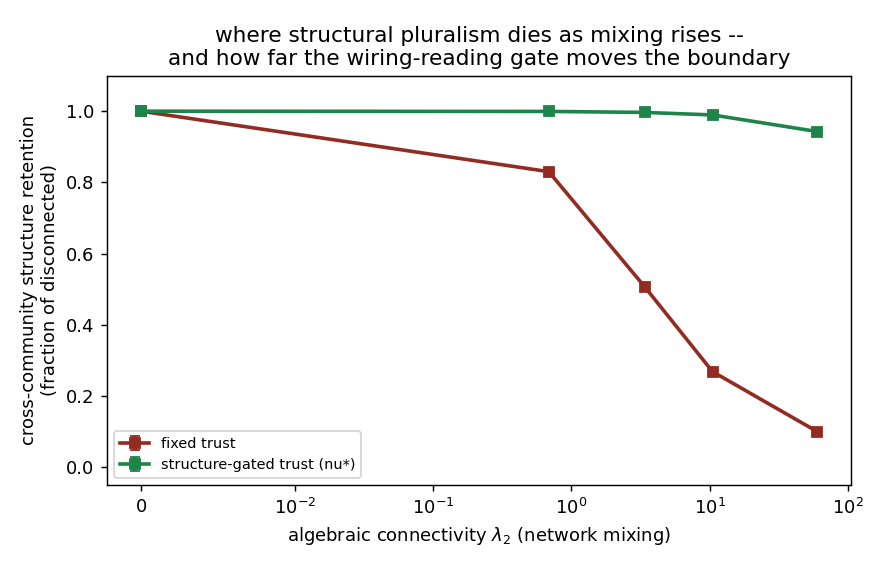
\includegraphics[width=0.6\linewidth]{fig_connectivity_boundary.png}
\caption{Where structural pluralism dies as mixing rises. $x$-axis: algebraic connectivity of
the contact graph; $y$-axis: surviving cross-community structure (fraction of the disconnected
benchmark). Fixed trust dilutes both wirings toward one compromise net as mixing rises; the
wiring-reading gate preserves the two learned structures even under dense contact. The
opinion-reading gate tracks the fixed-trust curve: the camps agree in means, so it never
fires.}
\label{fig:res-wiring}
\end{figure}

\paragraph{Scope, stated plainly.}
Three commitments bound the results. (i) Both gates are \emph{memoryless}: $\eta_k$ and
$\eta_{ij}$ are instantaneous functions of current surprise, so every school and schism reported is
metastability relative to a horizon, not a new fixed point---the contraction theorem owns
$t\to\infty$, and the lock-in rerun shows the trade directly: a harsher gate ($\nu_s{=}0.2$)
holds the boundary longer but leaves its own undoing unfinished at the same horizon, because
the lock and the merge run on the same clock. (ii) The schism control is normalized by the
pre-contact stance gap, since one uniform fusion step collapses the fixed-trust camps before
the first logged sample. (iii) Structure-as-precision-pattern is attention-driven in the
linear-Gaussian class (the Fisher deposit $H^{\!\top}\mathrm{diag}(w)H/\sigma^2$ never sees the
observation's value): a camp committed to a wiring the data do not support consolidates it
exactly as strongly as the supported camps do, so the wiring gate can protect a pluralism but
cannot tell a supported school from a merely committed one---the data's verdict on an
unsupported theory lives in the means, and in the strain and reliability reads that live on
them. This refuted our own prediction, and it is the right caveat on every wiring-gate claim.

% ======================================================================
% The crisis and discovery checks, derived from the ledger (+ the
% exploration-as-social-process mechanism readings at its tail).
% ======================================================================
% APPENDIX (v3): the crisis and discovery checks, derived from the ledger.
% \input from changing_networked_mind_v3.tex (after the operator appendix).
% Uses the main paper's macros (\Top, \KL, \Eq) and labels (eq:tilted,
% eq:bmr, eq:gamma, sec:structurelearning, sec:revision, tab:dials).
% ======================================================================

% ----------------------------------------------------------------------
\section{The crisis and discovery checks, derived from the ledger}
\label{app:crisis-discovery}
% ----------------------------------------------------------------------

The per-round loop of \S\ref{sec:model} contains two threshold events: the \emph{crisis check}
(when does an agent prune the protective edges and release the hub?) and the \emph{discovery
check} (when does it wake the unconceived node?). This appendix states exactly what each check
computes, derives both from the single objective the paper already carries, and lists the
modelling commitments that remain after the derivation. The aim is that nothing in the two
checks should read as a stipulated event: every acceptance is the model's own evidence weighed
on the model's own ledger, and everything that is \emph{not} derived is named as a commitment.

\subsection{One ledger for every structural move}

The bounded agent of \S\ref{sec:revision} revises its beliefs by minimizing
$\KL{q}{p(x\mid o,G)}-\lambda\,\Eq{q}{U^{\!\top}\!x}$ (Eq.~\ref{eq:tilted}): fidelity to the
honest posterior, traded against the value of where the commitments land, at temperature
$\lambda$. A structural move---pruning an edge, waking a node---changes both terms, so the same
objective scores the move:
\begin{equation}
\mathrm{score}(M\!\to\!\tilde M)
\;=\;
\underbrace{\Delta F}_{\text{log Bayes factor}}
\;+\;
\underbrace{\Delta G}_{\text{epistemic gain}}
\;+\;
\lambda\,\underbrace{\Delta U}_{\text{conviction value}},
\qquad
\text{accept}\iff \mathrm{score}>0,
\label{eq:ledger}
\end{equation}
with $\Delta F$ the evidence for the edited structure, $\Delta G$ the expected information gain
about any newly introduced latent (zero for a prune), and
$\Delta U = \Eq{q_{\tilde M}}{U^{\!\top}\!x}-\Eq{q_{M}}{U^{\!\top}\!x}$ the change in the
conviction-field value of the commitments. Equation~\eqref{eq:ledger} is not a new mechanism:
it is Eq.~\eqref{eq:tilted} evaluated at two structures and differenced. Both threshold events
of the simulation are instances of it.

\subsection{The crisis check is the ledger on a prune}

For a prune, every term of Eq.~\eqref{eq:ledger} is closed-form in the linear-Gaussian setting.
The evidence half is Bayesian model reduction (Eq.~\ref{eq:bmr}): writing the agent's
accumulated likelihood deposit as $J=\Pi-\Pi_0$, $j=h-h_0$, the Savage--Dickey identity scores
the swap of the prior $(\Pi_0,h_0)$ for the edge-$e$-reduced prior $(\Pi_0^{(e)},h_0^{(e)})$
under the same likelihood, and---this is the part the main text does not spell out---it
\emph{already exhibits the reduced posterior},
\begin{equation}
\Pi^{(e)} = \Pi_0^{(e)} + J,
\qquad
h^{(e)} = h_0^{(e)} + j ,
\end{equation}
so the value half costs one linear solve per candidate edge:
\begin{equation}
\Delta U_e \;=\; U^{\!\top}\!\bigl(\mu^{(e)}-\mu\bigr),
\qquad
\mu^{(e)} = \bigl(\Pi^{(e)}\bigr)^{-1}h^{(e)},\quad \mu = \Pi^{-1}h,
\label{eq:dU-prune}
\end{equation}
with $U=\Top u$ the agent's \emph{current} conviction field, read along its present couplings.
The crisis check is then exactly the ledger: edge $e$ is flagged iff
$\Delta F_e + \lambda\,\Delta U_e > 0$, and \emph{crisis} is the round at which both protective
belt edges are flagged, upon which the agent adopts the reduced prior composed over every edge
its own ledger flags (the hub released). Pruning a conviction-protective edge moves the
posterior mean away from the cherished commitments, so $\Delta U_e<0$ and the rule reproduces
the intuitive form ``the evidence must overcome $\lambda$ times the value the edge protects.''

A natural surrogate suggests itself here: the static threshold $\Delta F_e > \lambda\,v_e$ with
$v_e = |U_{\mathrm{parent}}|+|U_{\mathrm{child}}|$, the summed conviction magnitude at the
edge's endpoints---available without a solve, and with the
right \emph{form} (it is Eq.~\eqref{eq:ledger} with $\Delta U_e \equiv -v_e$). But it has the
wrong \emph{content}: $v_e$ is a static stand-in for a quantity the model can compute exactly,
so we compute it. The difference is not cosmetic, and its direction is itself informative:
because the reduced and full posteriors share the likelihood deposit, the mean displacement of
a prune---and with it $\lambda\,\Delta U_e$---\emph{shrinks as evidence accumulates}. A
data-rich paradigm is barely protected at the threshold; almost all of its persistence must
come from upstream, from the conviction gate that decides which evidence is allowed to
accumulate at all (Eq.~\ref{eq:gamma}). The static surrogate would quietly overstate threshold
protection; the exact ledger locates lock-in where the paper's results put it: gating plus
isolation, not a high bar at the moment of decision.

\subsection{The discovery check is the ledger on an expansion}

Expansion cannot be closed-form (\S\ref{sec:structurelearning}): a new node needs a real
inversion, and---Stanford's problem of unconceived alternatives---the agent cannot plan toward
a dimension it has not conceived. The discovery check therefore has exactly two parts, and only
two:

\begin{enumerate}
\item \textbf{Arrival.} Candidate proposals arrive at a Poisson rate $r$. This is the one
place a stipulated process enters, and it is a deliberate modelling commitment: a rate is the
maximally agnostic model of conceiving what one has not conceived. The proposal's
\emph{direction} is read from the model's own prediction errors: a hidden hub $b$ wired to the
visible nodes with couplings $c$ leaves, on marginalization, the rank-one footprint
$-cc^{\!\top}/\Pi_{bb}$, so the leading eigenvector of the windowed error second moment is the
best single-hub explanation of the residual. The window is an estimator horizon, not a gate.
\item \textbf{Acceptance.} The arrived proposal is accepted iff the \emph{model log Bayes
factor} of the bordered (hub-wired) model against the agent's current one is positive---that
is, iff the residual genuinely loads on the proposed hub, equivalently iff the immediate
Savage--Dickey prune of the new couplings would be rejected. The epistemic gain $\Delta G$ sits
on the ledger too, but on the other side of the move: being positive for \emph{any} new latent,
it is what pays for attempting the (in general expensive) inversion, and it cannot keep a hub
the data do not hold---an accept test that included it would wake on pure noise. Entertaining
is paid by curiosity; keeping is paid by evidence. One consequence is owned rather than hidden:
repeated looks give the Bayes factor a small false-discovery rate (rare
noise crossings of $\Delta F>0$ in the null world). We regard this as a feature of the honest
model---communities do occasionally adopt spurious structure---and its principled remedy is not
a reinstated threshold but the wake-then-prune cycle named in the limitations, in which a
spuriously woken node is pruned back by the same reduction that scored it.
\end{enumerate}

A tempting third part is deliberately absent: a \emph{trigger}, requiring the residual floor
(the eigenvalue above) to clear some height, perhaps for a sustained number of steps, before
the Bayes factor is consulted. Such a gate would duplicate the accept test's job with a free
constant---the Bayes factor already rejects proposals the residual does not support---and its
only principled reading, a budget on when to pay for the expensive inversion, is a statement
about real scientific communities rather than about this simulation, where the inversion is a
small log-determinant. The discovery check therefore has no tuned threshold: the Poisson rate
carries Stanford's commitment, the eigenvector carries the direction, and the ledger decides.
(The floor is still recorded as telemetry, because it is the visible signature of the residual
the old paradigm had been absorbing.)

\subsection{What remains a modelling commitment}

The derivation above leaves a short, explicit list of choices that are \emph{not} forced by the
formalism. We state them because the paper's claim that ``crisis, revolution and discovery are
threshold crossings of the model's own evidence'' is honest only if its boundary is drawn:

\begin{itemize}
\item \textbf{The belt conjunction.} ``Crisis'' is operationalized as \emph{both} named
mass-law edges flagged in the same round. The per-edge accept is derived; the conjunction over
those two edges is our operational definition of having eliminated the phlogiston mass-law
reading.
\item \textbf{The ordering --- a result, not a commitment.} The simulation attempts expansion
only after an agent's own crisis, but the ordering is enforced by the evidence rather than by
fiat: running the identical proposal + ledger pipeline for every pre-crisis agent at every step
(without applying it), the ledger rejects $13{,}180$ of $13{,}185$ pre-crisis agent-steps; the
five crossings are marginal ($\Delta F < 0.005$, two orders below the post-crisis acceptance
evidence) and are exactly the repeated-look false-positive rate owned above, whose remedy is
the wake-then-prune cycle (\S\ref{app:exploration-future}). The intact paradigm absorbs the
residual; there is nothing for the check to find until reduction exposes it.
\item \textbf{The Poisson rate $r$} (swept), the prediction-error \emph{window} (an estimator
horizon), a short \emph{warm-up} before reduction is permitted (an initialization guard), and
the released hub's self-precision are quantitative choices of the same standing as the other
dials of Table~\ref{tab:dials}.
\item \textbf{The closed-loop mechanisms' own commitments.} The mechanisms of
Appendix~\ref{app:closing} replace the constant rate, the one-shot accept and the static $u$
with inferred quantities, but import quantitative choices of their own: the
Hawkes kernel's parametric form ($\beta$, $\tau$, exponential memory)---the \emph{reading} of
the kernel as filtered social evidence is motivated below, its shape is chosen; the expiring
credit's geometric decay $\lambda_c$, a fixed-form surrogate for recomputing $\Delta G$ on the
current posterior; and the audit's grace and patience horizons. All are
Table~\ref{tab:dials}-class dials, swept or defaulted, never tuned against an outcome.
\end{itemize}

% ----------------------------------------------------------------------
\subsection{The rate, made principled (and the audit that pays its debts)}
\label{app:exploration-future}
% ----------------------------------------------------------------------

This subsection records the inferential readings that license the closed-loop mechanisms whose
quantitative results Appendix~\ref{app:closing} reports: the adequacy-driven rate, the social
excitation, the audit that the full ledger's acceptance rule makes necessary, and the accretion
dynamics behind the Lakatos result---together with what each leaves stipulated.

\paragraph{The adequacy belief, filtered.}
One explores at the rate one believes one's model is incomplete, and that belief has a licensed
likelihood: the residual floor the discovery check already records---the prediction error that
persists after every within-model update, whose persistence is therefore evidence about the
model \emph{class} rather than its parameters. The agent tracks it with a fixed-gain filter,
$s \leftarrow (1-\rho)\,s + \rho\cdot\mathrm{floor}$, the same exponential-forgetting form as
$\omega$ (and the fixed-gain limit of conjugate Gamma--Poisson updating under a drift prior on
the latent rate), and sets $r(t) = r_0 + \kappa_r \max(s - s_{\mathrm{ref}}, 0)$, capped at
$r_{\max}$. A persistent residual raises the agent's own arrival rate; a quiet model lets it
decay to the agnostic base. The clean waiting-time law of \S\ref{sec:res-pooling} does, as
anticipated, dissolve into a feedback system; the experiments therefore report realized
(effective) rates, and the matched-mean control of Appendix~\ref{app:closing} is what separates
``rate when needed'' from ``more rate.''

\paragraph{The social stream, and why its filter is a Hawkes kernel.}
Because the agents share one hidden world, model inadequacy has a common cause across the
community, and a trusted neighbour's discovery is evidence about one's \emph{own} adequacy
variable---the situation in which federated inference prescribes pooling
\citep{friston2023federated}. Filtering the neighbours' discovery events (a point process,
observed through the trust weights $T_{ij}$ the population already fuses over) under an
exponentially-correlated prior on the latent inadequacy yields a posterior intensity that is a
shot-noise process: a baseline plus a decaying bump per observed event. That is exactly the
linear self-exciting form of \citet{hawkes1971},
\begin{equation}
r_i(t) \;=\; r_0 \;+\; \sum_{j\in\partial i}\, T_{ij} \sum_{t_j < t} \beta\, e^{-(t-t_j)/\tau},
\end{equation}
with $t_j$ the neighbours' discovery times: $\beta$ the trust-scaled evidential weight of one
observed discovery, $\tau$ the assumed correlation time of inadequacy. The structural-proposal
channel the model already has is thereby promoted from carrying \emph{content} (which node to
wake) to also carrying \emph{momentum} (how eagerly to look)---a formal home for the observation
that revolutions arrive in waves---and the branching ratio becomes the model's measurable answer
to how much social excitement a revolution needs (Appendix~\ref{app:closing},
Fig.~\ref{fig:res-hawkes}). What the reading does not discharge: the kernel's parametric form is
chosen, and the excitation deposited by a wake that is later pruned back (below) is not
retracted---the community's excitement is an observation of the wake, not of the verdict.

\paragraph{The wake-then-prune audit.}
Accepting wakes on the full ledger $\Delta F + \Delta G > 0$ lets curiosity adopt structure the
data do not (yet) hold, so the acceptance rule itself creates the obligation to audit. The audit
re-asks the wake's own question every round: the bordered-model log Bayes factor of the agent's
\emph{current} (conditioned) beliefs against its \emph{pre-wake} anchor at the stored coupling
---not a Savage--Dickey prune of the wired prior, which would compare two priors and find the
hub favoured by construction, since the slot has no observation row and is held only by the
data's mean displacement along its pattern. The $k$-th audit's verdict is
\begin{equation}
\mathrm{verdict}_k \;=\; \Delta F_{\mathrm{now}} \;+\; \Delta G\,\lambda_c^{\,k},
\end{equation}
the wake's ledger with \emph{expiring} credit: epistemic gain pays for entertaining, but it is a
diminishing resource---information gain about a latent shrinks as the posterior over it
sharpens---so the geometric $\lambda_c$ is a fixed-form surrogate whose principled successor is
recomputing $\Delta G$ on the current hub posterior. A patience-length run of non-positive
verdicts (after a grace period covering post-wake consolidation) re-pins the slot to its exact
dormant form, and the agent may wake it again later: entertaining is paid by expiring curiosity,
keeping by evidence. Figure~\ref{fig:wakeprune} shows the cycle doing the false-discovery work
the commitments list above assigns it: in a null world that never shifts, the credit wakes hubs
in every agent and the audit re-pins every one of them; in the flip world the genuine hub is
woken everywhere and never pruned.

\begin{figure}[h!]
\centering
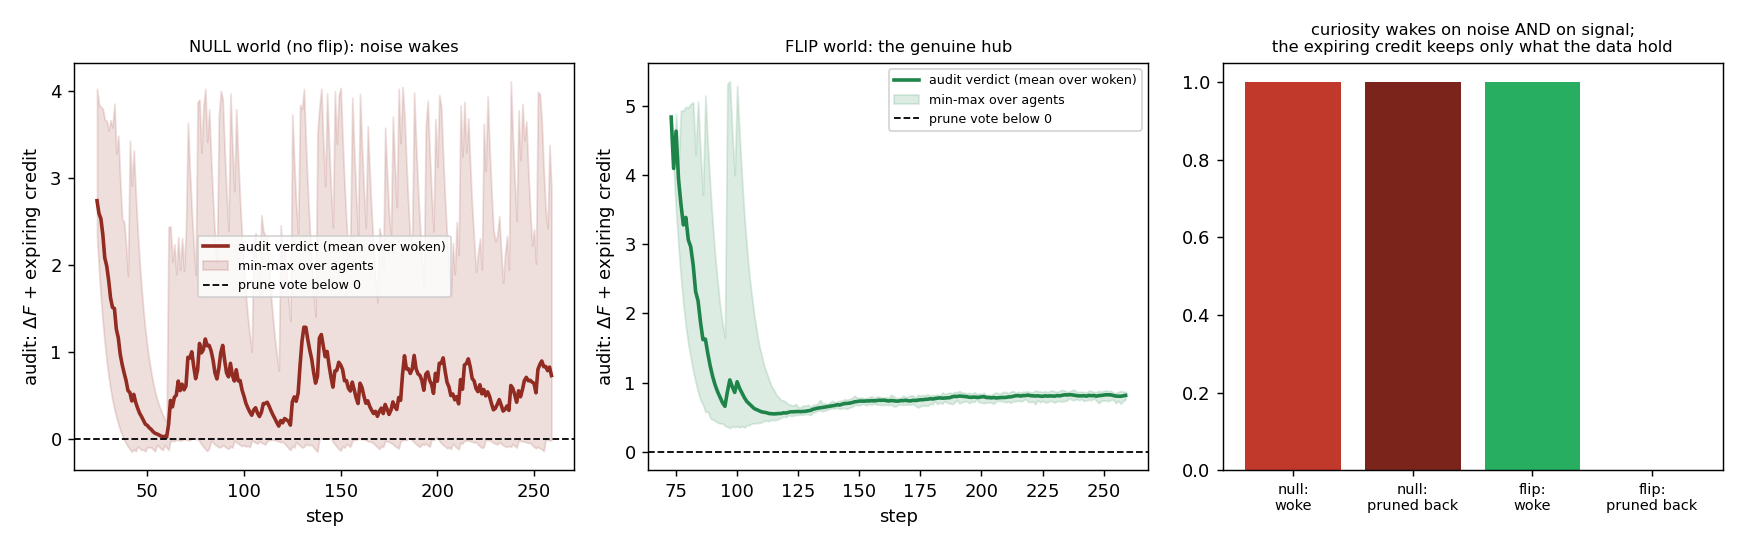
\includegraphics[width=\linewidth]{fig_wake_then_prune.png}
\caption{The wake-then-prune cycle controls the repeated-look false-discovery rate with no
threshold. \emph{Left:} null world (no regime shift)---the audit verdict (evidence plus
expiring credit) of every noise-woken hub decays below zero and the slot is re-pinned exactly.
\emph{Centre:} flip world---the genuine hub's verdict stays positive; the data take over before
the credit runs out. \emph{Right:} curiosity wakes structure in both worlds; the audit keeps
only what the data hold.}
\label{fig:wakeprune}
\end{figure}

\paragraph{Value accretion (the Lakatos closure).}
The conviction source $u$, exogenous and static in the baseline, gains slow dynamics:
per node, $u_{\mathrm{eff}} = u\,(1+g)$ with
$g \leftarrow \mathrm{clip}(g + \epsilon\,e - \delta\,g,\,0,\,g_{\max})$ and $e$ the agent's own
entrenchment (the diagonal of its accumulated evidence deposit $\Pi-\Pi_0$, max-normalized)---
self-evidencing made slow \citep{hohwy2016}: value flows toward the commitments the programme's
own data have entrenched, and through $U=\Top u$ and the gate of Eq.~\eqref{eq:gamma} a maturing
programme increasingly silences its own disconfirming channels. The clip bounds the
accretion--gate feedback loop. Figure~\ref{fig:lakatos} shows the resulting phase picture: gain
accreting over the run, the realized gate climbing with $\epsilon$, and conversion at the
lock-in boundary falling---progressive and degenerating problemshifts as dynamics
(Appendix~\ref{app:closing}).

\begin{figure}[h!]
\centering
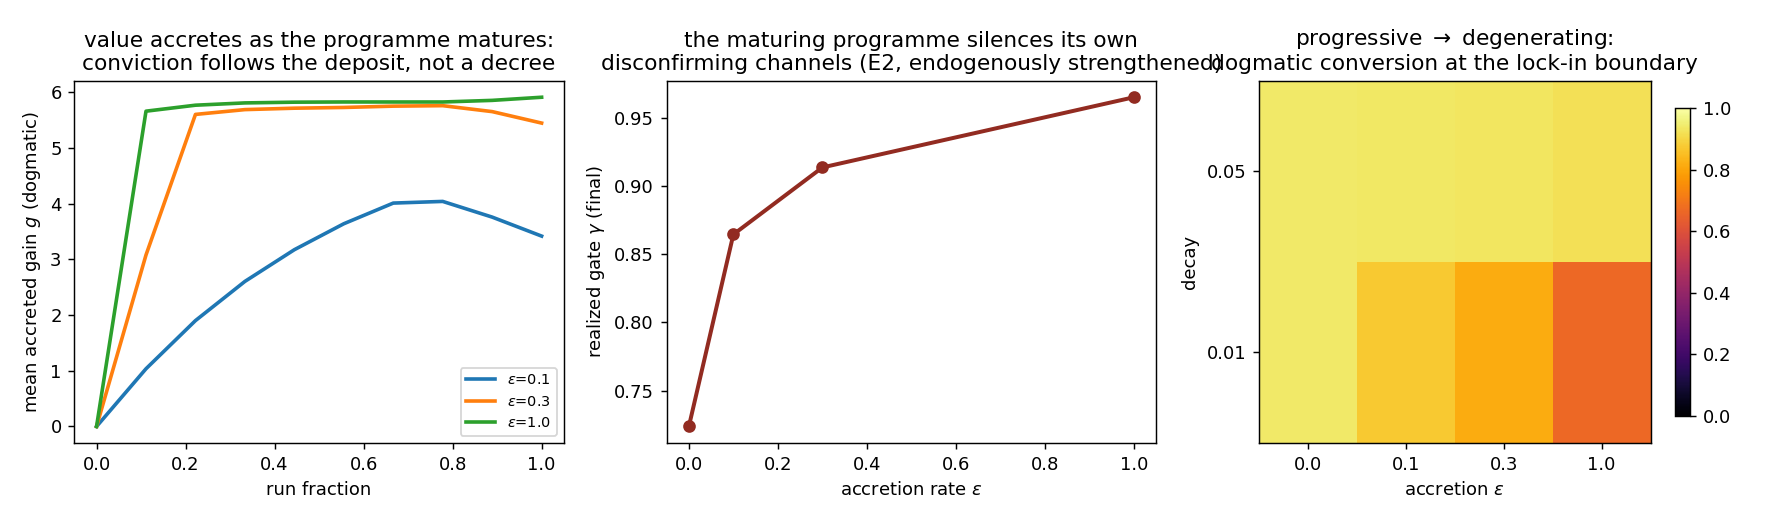
\includegraphics[width=\linewidth]{fig_lakatos.png}
\caption{Dynamic conviction (Lakatos, run forward). \emph{Left:} the accreted gain $g$ grows as
the programme matures---conviction follows the agent's own evidence deposit, not a decree.
\emph{Centre:} the realized self-silencing gate $\gamma$ strengthens with the accretion rate
$\epsilon$. \emph{Right:} dogmatic-community conversion at the lock-in boundary over the
$(\epsilon,\,\mathrm{decay})$ plane: a programme that matures into conservatism delays its
supersession---and still loses to connection.}
\label{fig:lakatos}
\end{figure}


% ======================================================================
\section{Closed-loop mechanisms: quantitative results}
\label{app:closing}
% ======================================================================

The baseline model holds four quantities fixed that admit treatment as beliefs or protocols: the
proposal rate, the acceptance of a wake, the conviction source $u$, and the pooling rule. The
inferential readings that license each mechanism are derived in
Appendix~\ref{app:exploration-future}; this appendix reports what each does to the population
results. Every mechanism defaults to ``off''---constant rate, one-shot accept, static $u$, delta
pooling---reproducing the baseline exactly, and each comparison below is run against that
baseline with its own control.

\paragraph{The rate as a posterior over model adequacy.}
The agent tracks its residual floor---the leading eigenvalue of the windowed prediction-error
second moment, the error no within-model update can absorb---with a fixed-gain filter
$s \leftarrow (1-\rho)\,s + \rho\cdot\mathrm{floor}$ and reads its proposal rate off the
posterior, $r(t) = r_0 + \kappa_r \max(s - s_{\mathrm{ref}}, 0)$. The result
(Fig.~\ref{fig:res-rateposterior}) has the signature a posterior should have and a dial cannot:
flat at $r_0$ through normal science, surging after the agent's own crisis exposes the residual
(to an effective $0.34$ from $r_0=0.01$), and decaying once the woken node explains it. The
crisis-to-discovery delay falls from $55$ to $29$ steps---but the control that matters is the
fixed rate it \emph{matches}: a constant-rate agent given the adaptive run's realized mean rate
achieves the same delay ($27$ steps). The gain is not more exploration; it is exploration when
the agent's own evidence calls for it. Stanford's constraint survives: only the \emph{propensity
to look} is inferred, never a direction.

\begin{figure}[h!]
\centering
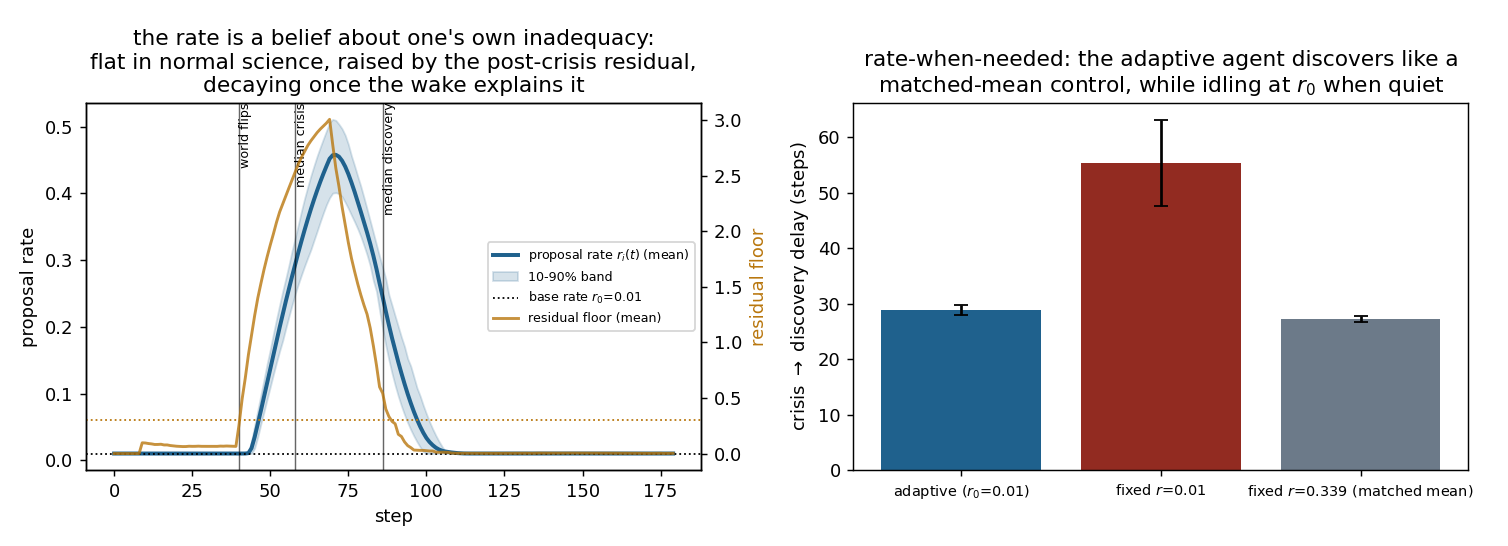
\includegraphics[width=\linewidth]{fig_rate_posterior.png}
\caption{The proposal rate as a posterior over model adequacy. \emph{Left:} the per-agent rate
(blue, mean and 10--90\% band) is flat at the base rate $r_0$ through normal science, rises with
the post-crisis residual floor (amber, right axis)---the evidence of model-class inadequacy the
within-model updates cannot absorb---and decays once the woken node explains it. \emph{Right:}
crisis-to-discovery delay. The adaptive agent (left bar) matches a fixed-rate control given its
realized mean rate (right bar) while idling at $r_0$ when the model is adequate: the gain is
rate-when-needed, not more rate.}
\label{fig:res-rateposterior}
\end{figure}

\paragraph{Social excitation rescues the staggered discovery.}
Filtering neighbours' discovery events through the trust weights, under an
exponentially-correlated prior on the latent inadequacy, yields a posterior intensity of exactly
the linear self-exciting (Hawkes) form \citep{hawkes1971},
\begin{equation}
r_i(t) \;=\; r_0 \;+\; \sum_{j\in\partial i} T_{ij} \sum_{t_j<t} \beta\, e^{-(t-t_j)/\tau},
\label{eq:hawkes}
\end{equation}
with $t_j$ the neighbours' discovery times, $\beta$ the trust-scaled evidential weight of one
observed discovery, and $\tau$ the assumed correlation time of inadequacy
(Appendix~\ref{app:exploration-future}). Under Eq.~\eqref{eq:hawkes} the first discovery raises
the whole neighbourhood's propensity to look; the cascade compresses the community's wakings from
a dispersion of $64$ steps to $2$, and---because survival is \emph{completeness}-driven (a single
still-pinned peer holds the fused slot precision enormous for every neighbour)---the completed
cascade lets the anchored couplings consolidate. Survival rises monotonically in $\beta$ from
exactly zero at $\beta=0$ to $0.88$--$0.95$ at $\beta=1.5$ across base rates
$r_0\in\{0.005,0.01,0.02\}$ at which an unexcited community essentially never completes
(Fig.~\ref{fig:res-hawkes}; 32 seeds per cell). The branching ratio of Eq.~\eqref{eq:hawkes} is
the model's quantitative answer to how much social excitement a revolution needs. One qualifier:
survival is completeness-driven and therefore horizon-bound---a constant-rate community given a
high enough rate and a long enough horizon also completes its cascade; what excitation adds is
the mechanism by which a community reaches near-simultaneity at rates serendipity alone
essentially never does.

\begin{figure}[h!]
\centering
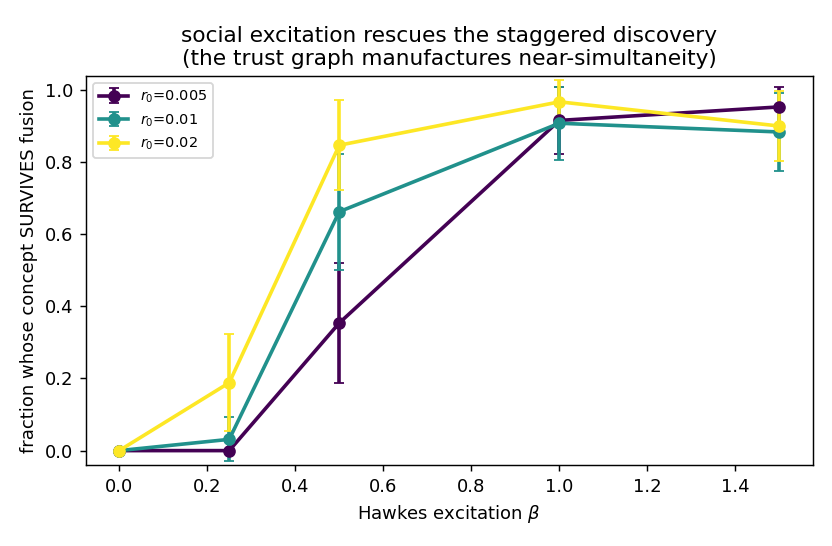
\includegraphics[width=0.62\linewidth]{fig_kuhn_hawkes.png}
\caption{Social excitation rescues the staggered discovery (sweep panel E, 32 seeds per cell).
Fraction of the open community whose oxygen concept survives fusion, versus the excitation
$\beta$ of Eq.~\eqref{eq:hawkes}, at three base rates. At $\beta=0$ (the constant rate) survival
is exactly zero: staggered wakings are crushed one at a time. Excitation compresses the
community's wakings in time, the cascade completes, no pinned peer remains in the fusion average,
and survival rises to $0.88$--$0.95$---the near-simultaneity that survival requires, manufactured
by the community itself.}
\label{fig:res-hawkes}
\end{figure}

\paragraph{The audited wake-then-prune cycle.}
Accepting wakes on the full ledger $\Delta F + \Delta G > 0$ lets curiosity adopt structure the
data do not yet hold, and the audit of Appendix~\ref{app:exploration-future} pays that debt: in a
null world that never shifts, curiosity wakes structure in $100\%$ of agents and the audit
re-pins $100\%$ of those wakes, exactly; in the flip world the genuine hub is woken everywhere
and never pruned (Fig.~\ref{fig:wakeprune}). Two companion measurements close two more
commitments. Widening the search---three eigen-hub candidates, each with its own dormant slot,
plus the three largest residual couplings, $1{,}140$ candidates priced on the same ledger---does
not dilute discovery: the true cause wins $53$ of $60$ acceptances (median cosine $0.999$ against
the rank-one baseline). And running the identical discovery check \emph{before} each agent's
crisis, at every step, the ledger rejects $13{,}180$ of $13{,}185$ pre-crisis agent-steps: the
crisis-before-expansion ordering is enforced by the evidence, not by fiat---the intact paradigm
absorbs the residual, so there is nothing for the check to find until reduction exposes it.

\paragraph{Value accretion (Lakatos, run forward).}
Letting $u$ accrete onto the commitments the agent's own evidence deposit has entrenched
(Appendix~\ref{app:exploration-future}) closes the loop through the gate of
Eq.~\eqref{eq:gamma}: a maturing programme increasingly silences its own disconfirming channels
($\gamma$ climbs from $0.72$ to $0.97$ as $\epsilon$ rises), conversion at the lock-in boundary
falls from $0.94$ to $0.67$, and at very weak coupling the dogmatic community's conversion is
\emph{delayed} roughly $2.2$-fold rather than prevented (Fig.~\ref{fig:lakatos}). Conviction that
grows from the inside still loses to connection: it buys the old paradigm time, not immunity---a
fair gloss of a degenerating problemshift.

\paragraph{The mechanisms compose.}
With the adequacy-posterior rate, social excitation, the expiring-credit audit, abstention
pooling and value accretion all enabled in one population, the full arc still runs---crisis at
$t\approx67$, discovery at $t\approx69$, the rate surging $0.02\to0.77$ and decaying back to
base, zero false prune-backs, concept survival complete, and the never-shifting null world silent
in every channel. No mechanism breaks another, because none adds a new objective: each routes a
quantity the ledger already computes---residual, epistemic gain, evidence, deposit---back into a
parameter that had been a constant.

\end{document}
